\documentclass[12pt]{article}
\usepackage{graphicx} % Required for inserting images
\usepackage[margin=1.25in]{geometry}
\usepackage{fancyhdr}
\usepackage{biblatex} %Imports biblatex package
\usepackage{amsfonts}
\usepackage{amsmath}
\usepackage{float}
\usepackage{subfig}
\usepackage{caption}
\addbibresource{references.bib} %Import the bibliography file
\graphicspath{ {./images/} } % Directory where figures are stored 


\title{Thesis}
\author{Max Yuan}
\date{December 2023}


\pagestyle{fancy}
\fancyhf{} % clear all header and footer fields
\fancyhead[R]{Max Yuan} % right side header
\fancyfoot[C]{\thepage} % center footer
\renewcommand{\headrulewidth}{0.4pt} % header line width
\renewcommand{\footrulewidth}{0pt} % no footer line

% custom comment command
\newcommand{\comment}[1]{}


\begin{document}

% Title Page
\begin{titlepage}
    \thispagestyle{empty} % No headers or footers on title page
    \centering
    \vspace*{\stretch{1}}
    \Huge
    Using Deep Q-Learning to Play Two-Player Yahtzee\\
    \vspace{10mm}
    \Large
    Max Yuan\\
    Advisor: Professor James Glenn\\
    \vspace{10mm}
    Yale University\\
    December, 2023
    \vspace*{\stretch{2}}
\end{titlepage}

% Abstract Page
\newpage
\begin{abstract}
\noindent
Yahtzee, a dice game based on poker, can be played either by yourself or with multiple players. Today's computers can handily solve the single-player version of Yahtzee, but the multiplayer version of the game is too complicated to be solved—optimal play must be approximated through other means. This thesis explores the development and performance of a Deep Q-Learning Network (DQN) agent designed to learn and play the game of two-player Yahtzee. The objective is to create an AI agent that not only understands the basic rules of Yahtzee but also learns strategy and improves as much as possible. The DQN agent is trained through reinforcement learning, where it learns optimal strategies by playing numerous games against various opponents, including two deterministic rule-based agents and a randomized agent. The deterministic rule-based agents are designed to play the optimal solitaire strategy and a greedy solitaire strategy, which are derived from the findings of previous literature and rebuilt in Python in this thesis.

Nine different variants of the DQN agent are trained and evaluated against the three aforementioned opponents. The variants differ in their reward functions, training opponents, and training length. Ultimately, the best of the nine variants was not able to match the performance of the optimal solitaire agent, scoring an average of 159 points against the optimal agent with a winrate of 6\%, but it did quickly learn the rules of Yahtzee and make significant improvements over the random agent. With easily customizable DQN and Yahtzee environment implementations, this thesis provides a solid foundation for future research into improving the DQN agent's performance to match or exceed the optimal solitaire agent.
\end{abstract}

\tableofcontents

\newpage
\section{Introduction}
% Your introduction content here
Yahtzee is a popular dice game that combines both strategy and luck. One interesting aspect of the game is that it can be played either by yourself or with multiple players. In the solitaire version of the game, the goal is to maximize your score, while in the multiplayer version of the game, the goal is to score higher than your opponents.

At first glance, it might seem like maximizing your expected score is optimal for both versions of the game. However, the optimal solitaire strategy is no longer optimal when you move to the multiplayer game because it is irrelevant how much you beat your opponents by—winning by 1 point is equivalent to winning by 50 points. Thus, if you are ahead early, it might be in your best interest to play conservatively to obtain a good enough score with a higher probability than gunning for your maximum possible expected score. On the other hand, if you are behind, then it might be in your best interest to play aggressively for the highest possible score despite the risk.

Yahtzee can be "solved" (i.e. calculating the best action for every possible state of the game) using the Markov Decision Process. In the solitaire version of the game, the number of states is low enough for today's computers to perform this calculation, and Professor James Glenn uses dynamic programming to solve solitaire Yahtzee in his paper, "An Optimal Strategy for Yahtzee" \cite{glenn}. However, when you add players to the game, the number of states increases exponentially. In this paper, I will be specifically exploring the two-player version of the game, but even still, there are too many states to calculate using dynamic programming. Instead, I will be using a Deep Q-Learning Network (DQN) agent to both grasp the fundamental rules of Yahtzee and learn to play good moves. I will also develop 3 agents playing various solitaire strategies to evaluate the variants of my DQN agent against: a random agent, a greedy agent, and an optimal agent.

Existing research on applying reinforcement learning techniques to multiplayer Yahtzee is limited. One group out of Stanford University applied the MAXQ Q-Learning approach, a form of hierarchical learning, to two-player Yahtzee \cite{kang}. However, their agent did not consider the opponent's scorecard when making decisions, and its final performance was not strong. Their best-performing agent averaged a score of 129.58. Another attempt at applying reinforcement learning to Yahtzee was made by Dion Häfner, who applied the Advantage Actor-Critic (A2C) algorithm to two-player Yahtzee \cite{hafner}. His agent ultimately performed quite well, achieving a mean score of around 236. We will see how my agent using Deep Q-Learning compares to these previous attempts.

\section{Methods}

\subsection{Rules}

In a game of Yahtzee, players alternate turns until everyone has filled all 13 categories on their scorecard. A player's turn starts with them rolling five traditional six-sided dice. The player can then choose any combination of the five dice to reroll, and they get up to two rerolls per turn. At any point, the player can choose to score their current dice combination in one of the empty categories on their scorecard. Once a category is filled, it cannot be changed and stays filled until the end of the game. Points are awarded to the 13 categories based on the following rules:

\begin{itemize}
    \item \textbf{Upper Section:} The upper section of the scorecard consists of six categories, each corresponding to a different dice value on a six-sided dice. The score for each category is the sum of all dice showing that value. For example, if a player has three 2s and two 5s, they can choose to score 6 points in the 2s category or 10 points in the 5s category. Furthermore, if the sum of the scores in the upper section is 63 or higher, the player gets a 35-point bonus.
    \item \textbf{Lower Section:} The lower section of the scorecard consists of seven categories, each corresponding to a different scoring combination. The score for each category is determined by the following rules:
    \begin{itemize}
        \item \textbf{Three of a Kind:} Sum of all five dice if there are at least three dice with the same value. 0 points otherwise.
        \item \textbf{Four of a Kind:} Sum of all five dice if there are at least four dice with the same value. 0 points otherwise.
        \item \textbf{Full House:} 25 points if there are three dice with the same value and two dice with another value. 0 points otherwise.
        \item \textbf{Small Straight:} 30 points if there are four dice with consecutive values. 0 points otherwise.
        \item \textbf{Large Straight:} 40 points if there are five dice with consecutive values. 0 points otherwise.
        \item \textbf{Yahtzee:} 50 points if all five dice have the same value.
        \item \textbf{Chance:} Sum of all five dice.
    \end{itemize}
\end{itemize}

\noindent
One variation of Yahtzee allows players to earn a bonus of 100 points if they score a Yahtzee after already scoring a Yahtzee. This variation with "Yahtzee Bonuses" is not considered in this paper. 

\subsection{Developing the Optimal Solitaire Agent}
In order to test the performance of my DQN agent against an agent playing the optimal solitaire strategy, we need to first solve solitaire Yahtzee and obtain the expected future score for each state. Taking inspiration from Glenn's aforementioned paper, "An Optimal Strategy for Yahtzee" \cite{glenn}, our Yahtzee game state will consist of the following:

\begin{itemize}
    \item \textbf{Scorecard:} The player's scorecard represented as a bitmask of length 13. Each bit is 1 if the corresponding category is filled and 0 otherwise. Since there are 13 categories, are bitmask will range from $0$ to $2^{13} - 1$, which can seamlessly be used to index into our dp array of expected future scores.
    \item \textbf{Upper Section Score:} The sum of the scores in the upper section of the scorecard. Since the upper score bonus threshold is 63, we can represent this as a number from $0$ to $63$. Anything above 63 is essentially equivalent to 63 in terms of expected future score.
\end{itemize}

\noindent
In order to calculate the expected future score for a given game state, we need to consider every possible action that we can take in a turn starting with that game state. Our Yahtzee turn state will consist of the following:

\begin{itemize}
    \item \textbf{Roll Number:} The current roll number represented as a number from $1$ to $3$. This is used to keep track of how many times we have rolled the dice in a turn.
    \item \textbf{Dice:} The current dice combination represented as an integer tuple of length six. $Dice[index]$ represents how many dice are showing $index + 1$ pips (since the tuple is 0-indexed). For example, if we have three dice showing two pips and two dice showing five pips, then our $Dice$ tuple would be (0, 3, 0, 0, 2, 0).
\end{itemize}

\noindent
At the start of a turn, the roll number is always one, and we could have any dice combination. Then, we can either choose a category immediately or reroll some combination of the dice. If we reroll, then our roll number increments to two, and we once again have the choice of rerolling some combination of the dice or choosing a category. If we reroll again, then our roll number increments to three, and we must choose a category to score. When we choose a category to score, our turn ends, and we get a new game state. Otherwise, when we reroll the dice, we get a new turn state.

We can calculate the expected future score for a given game state by taking the weighted average of the expectations of all the turn states we could be in after the first roll. The expectations of those turn states with $Roll Number = 1$ is the $max$ between the weighted average of the expectations of all possible turn states from rerolling all possible subsets of the dice and the highest scoring unused category plus the expected future score of the game state we get from choosing that category. The expectations of those turn states with $Roll Number = 2$ is calculated similarly, and the expectations of those turn states with $Roll Number = 3$ is simply the $max$ of the highest scoring unused category plus the expected future score of the resulting game state.

The dependency of game states and turn states on future game states and turn states lends itself nicely to dynamic programming. To ensure that a future game state or turn state has definitely been calculated by the time it is needed, we iterate through the states in the following orders:

\begin{itemize}
    \item \textbf{Game States:} Iterate through the scorecard bitmasks from bitmasks with more set bits to bitmasks with fewer set bits. Specifically, we start with the bitmask with all 13 bits set to 1, move on to all bitmasks with 12 bits set to 1, $etc.$ For the upper section score, we simply iterate from 63 down to 0. 
    \item \textbf{Turn States:} Iterate through the roll number from $3$ to $1$ and iterate over all possible dice combinations for each roll number.
\end{itemize}

\noindent
In his paper, Glenn observes that a substantial number of the game states are unreachable and can be skipped \cite{glenn}, saving precious computational time. For example, if our scorecard bitmask has only 1s filled out, then it is impossible for the upper section score to be anything higher than 5. All game states with a bitmask of 1 and an upper section score higher than 5 can be skipped. The same dynamic programming algorithm he presents is implemented in this paper to prune out over 30\% of game states.

To further speed up the dynamic programming computation, the following values will be precomputed:

\begin{itemize}
    \item \textbf{Dice Rolls:} An array of all possible dice combinations for a number of dice. For example, $DiceRolls[4]$ is an array of all possible dice combinations for five dice (five because the array is 0-indexed). This array is helpful for iterating over all possible initial dice rolls.
    \item \textbf{Dice To Keep:} A map from a dice combination to an array of all possible dice combinations that could be kept. For example, $DiceToKeep[(0, 3, 0, 0, 2, 0)]$ is an array of all possible dice combinations that could be kept if we have three dice showing two pips and two dice showing five pips. The tuple (0, 1, 0, 0, 1, 0) is an example of a dice combination that could be kept.
    \item \textbf{Scores:} A map from a dice combination and category to the score of that category. For example, $Scores[(0, 3, 0, 0, 2, 0)][1]$ is the score of the 2s category if we have three dice showing two pips and two dice showing five pips. The score would 6.
    \item \textbf{Dice Probabilities:} A map from a dice combination to the probability of that dice combination. For example, $DiceProbabilities[(0, 3, 0, 0, 2, 0)]$ is the probability of getting three dice showing two pips and two dice showing five pips. The probability would be $\frac{5!}{6^{5} * 3! * 2!}$.
    \item \textbf{Rerolled Dice Combo:} A map from a dice combination that we are keeping to an array of all possible dice combinations that could result from rerolling along with their probability. For example, $RerolledDiceCombo[(0, 3, 0, 0, 1, 0)]$ is an array of all possible dice combinations that could result from rerolling if we kept three dice showing two pips and one dice showing five pips. The tuple (1, 3, 0, 0, 1, 0) is an example of a dice combination that resulted from rolling a dice showing one pip, and its corresponding probability would be $\frac{1}{6}$.
    \item \textbf{Unused Categories:} An array of all unused categories for a given scorecard bitmask. For example, $UnusedCategories[2^{13} - 2]$ is an array of all unused categories for a scorecard with bits 1111111111110. The array would be [0], meaning that only the "1s" category is unused.
    \item \textbf{Turn Actions:} A map from a turn state to all the possible actions that can be taken. If the roll number is three, then the 13 categories are the only possible actions. Otherwise, if the roll number is less than 3, then the dice combinations that we get from $DiceToKeep$ indexed on the turn state's dice are included as other possible actions.
\end{itemize}

\noindent
Upon completing the dynamic programming computation and obtaining the expected future score for each game state, we can now create an agent to play the optimal solitaire strategy in simulated 2-player Yahtzee games. My Python implementation of Yahtzee will give the agent the current game state with their scorecard as well as their current turn state with their dice combination and roll number. The agent will then find the action with the highest expected future score and return that action. While the table of expected future scores for all game states takes up a manageable 4.8MB of memory, the table of expected future scores for all turn states takes many many gigabytes of memory, so our agent will have to recalculate the expected future score of turn states on the fly. This is not a problem, however, since the agent only has to calculate the turn states for one game state, which can be done in fractions of a second. Furthermore, the recalculated expected future scores of turn states are cached, speeding up performance as the agent plays more games.

\subsection{Developing the Greedy Solitaire Agent}
Fortunately, the greedy solitaire agent reuses the work that has been done to implement the optimal solitaire agent. Like the optimal agent, it receives the current game state and turn state. The greedy agent also has to loop over all possible actions and recalculate their expected future scores. However, while the optimal agent takes into account all future game states into its expected future score calculation, the greedy agent only takes into account the score that it will receive when it chooses a category at the end of the turn. Specifically, the optimal agent will add the expected future score of the new game state when scoring a category; the greedy agent will add zero.

\subsection{Developing the Random Agent}
The random agent simply gets the possible actions for the given turn state using the precomputed value $TurnActions$ and then filters out the categories that have already been filled out according to the scorecard bitmask from the given game state. It then randomly chooses one of the remaining actions to play.

\subsection{Developing the DQN Agent}
Deep Q-Learning (DQN) is a reinforcement learning algorithm that combines Q-Learning with deep neural networks. The goal of Q-Learning is to find a function 

\begin{center}
    $Q^*: State \times Action \rightarrow \mathbb{R}$
\end{center}

\noindent
$Q^*$ tells us our reward for a given state and action. We could then use $Q^*$ to construct the optimal policy $\pi^*$, where

\begin{center}
    $\pi^*(s) = \underset{a \in A}{argmax} \; Q^*(s, a)$
\end{center}

\noindent
However, since the state space is far too large for us to know $Q^*$, we instead use function $Q$ that approximates $Q^*$, where

\begin{center}
    $Q(s, a) = r(s, a) + \gamma \; \underset{a' \in A}{max} \; Q(s', a')$
\end{center}

\noindent
$r$ is the reward function, $\gamma$ is the discount factor, and $s'$ is the next state.

The core idea behind DQN is to use a neural network as a function approximator for $Q$ to estimate the Q-values, which are indicative of the quality of a particular action taken in a given state. This approach allows the agent to make decisions based on complex, high-dimensional input states. The DQN agent learns to optimize its behavior by interacting with the following environment and observing the resulting rewards or penalties.

\subsubsection{Yahtzee Gymnasium Environment}
My Yahtzee Gymnasium environment is a custom implementation of the Yahtzee game, designed to be compatible with the OpenAI Gym framework. The OpenAI Gym framework makes it easy to develop and test reinforcement learning algorithms by providing a standardized interface for interacting with environments. The exposed methods of a gym environment include:

\begin{itemize}
    \item \textbf{Constructor (init):} Initializes the environment and returns the initial state. In the case of Yahtzee, the initial state includes:
    \begin{itemize}
        \item an instance of our custom Yahtzee game
        \item parameters for the reward system
        \item a flag to turn on debug mode, which prints out data during training
        \item the observation space
        \item the action space
    \end{itemize}
    \item \textbf{sample\textunderscore action:} A function that samples a random action from the action space.
    \item \textbf{step:} A function that takes in an action and returns the next state, reward, and whether the game is over.
    \item \textbf{reset:} A function that resets the environment and returns the initial state.
\end{itemize}

\noindent
The observation space for this Yahtzee environment is a complex combination of various game elements, including:

\begin{itemize}
    \item Bitmask representation of the player's scorecard
    \item The player's upper score normalized to be between 0 and 1 by dividing by 63
    \item Bitmask representation of the opponent's scorecard
    \item The opponent's upper score normalized to be between 0 and 1 by dividing by 63
    \item The difference between the player's score and the opponent's score normalized to be between -1 and 1 by dividing by 375
    \item The current roll number as a one-hot encoding
    \item The count of each dice value normalized to be between 0 and 1 by dividing by 5
\end{itemize}

\noindent
The action space for this Yahtzee environment is a set of 23 possible "meta-actions" represented as a number from 0 to 22. The meta-actions are as follows:

\begin{itemize}
    \item \textbf{0-5:} Go for a specific dice value. For example, if the meta-action is 3, then the agent will reroll all dice except for the ones showing four pips.
    \item \textbf{6:} Go for as many of a specific dice value as possible. This is useful for going for three-of-a-kind, four-of-a-kind, and Yahtzee. The agent will reroll all dice except for the ones showing the most common value.
    \item \textbf{7:} Go for a straight. The agent will reroll all dice except for the ones that are part of the longest consecutive sequence.
    \item \textbf{8:} Go for a full house. The agent will reroll all dice except for the ones showing the two most common values.
    \item \textbf{9:} Go for a chance. The agent will reroll all dice that are not showing four, five, or six pips in an attempt to get a high sum.
    \item \textbf{10-22:} Go for a specific category. For example, if the meta-action is 12, then the agent will choose the 3s category to score.
\end{itemize}

\noindent
Originally, the action space was a set of 45 possible actions, where the first 32 actions were all the possible combinations of the five dice to reroll (including the option to not reroll any dice), and the last 13 actions were all the possible categories to score. However, this action space was ineffective because the same reroll action would have different behaviors depending on the current dice combination. For example, if the agent chose to reroll the first two dice, that one action would have wildly different outcomes depending on if the first two dice were both showing one pip or if they were both showing six pips. The meta-actions solve this problem by allowing the agent to shoot for a specific dice combination or category without having to specify the exact dice to reroll.

\subsubsection{Reward Function Variants}
The problem with deciding on a reward function for 2-player Yahtzee is that the ultimate reward—whether or not the agent won—is only given at the end of the game. The intermediate actions of which dice to reroll and which categories to score contribute to the end goal of winning the game, but they themselves do not give any immediate rewards. If the only reward the agent was exposed to was the reward at the end of the game, it would be extremely inefficient for the agent to learn the intermediate strategies that lead to winning the game. Thus, we need to design a reward function that gives the agent immediate rewards for taking good actions.

I ultimately settled on an intermediate reward function that compares the score the agent obtained from choosing a category to the average score an optimal agent would have obtained from choosing that category. To obtain the average category score achieved by an optimal solitaire player, I had my optimal solitaire agent play 1000 games and obtained the following rough averages:

\begin{center}
    \begin{tabular}{ |c|c| }
        \hline
        Category & Average Score \\
        \hline
        1s & 1.861 \\
        2s & 5.366 \\
        3s & 8.676 \\
        4s & 12.116 \\
        5s & 15.65 \\
        6s & 19.488 \\
        3 of a kind & 22.344 \\
        4 of a kind & 12.897 \\
        Full house & 23.125 \\
        Small straight & 29.43 \\
        Large straight & 33.12 \\
        Yahtzee & 17.0 \\
        Chance & 22.286 \\
        \hline
    \end{tabular}
\end{center} 

\noindent
If the agent's action is to choose an unused category, then the reward is the difference between the agent's score and an optimal agent's average score for that category divided by 10. I divide by 10 to scale down the intermediate rewards and ensure that it does not overpower the final reward of winning or losing the game. If the agent's action is to reroll the dice, then the reward is 0. If the agent's action is to choose a category that has already been filled out, then the reward is a severe -10 to punish it.

The reward function at the end of the game is also not as straightforward as it seems. Take for example the naive reward function where the agent gets 1 if it wins and -1 if it loses. When trained against a strong opponent like my optimal solitaire agent, the DQN agent will lose every single game and continue getting rewards of -1, which is not very instructive. Against a weak opponent like my random agent, the DQN agent will win every single game and continue getting rewards of 1, which is also not very instructive when the ultimate goal is to beat the optimal solitaire agent. Thus, in an attempt to find a better reward function, the following variants will be tested:

\begin{itemize}
    \item \textbf{Naive:} The agent gets 1 if it wins, -1 if it loses, and 0 if it draws.
    \item \textbf{Gradient:} Instead of getting the same reward when losing regardless of the margin, the agent gets a reward proportional to the margin of defeat. The reward for losing is the score difference divided by 100. Winning and drawing still give rewards of 1 and 0 respectively because the margin of victory does not matter, and the purpose of the gradient when losing is to encourage the agent to lose by as little as possible while it is still learning.
    \item \textbf{Fixed:} A score goal of 110 is set for the agent to achieve. The agent gets 1 if it achieves the score goal, -1 if it does not, and 0 if it draws. 110 was chosen as an intermediate score value between random performance and optimal performance. Note that the opponent's score is not taken into account when calculating the reward.
    \item \textbf{Moving Average:} Instead of a fixed score goal, the score goal moves with the agent's performance. The minimum score goal is still 110, but as the agent learns and gets better, the score goal becomes 20 points higher than the agent's average score over the last 100 games. The agent gets 1 if it achieves the score goal, -1 if it does not, and 0 if it draws. Again, the opponent's score is not taken into account when calculating the reward.
\end{itemize}

\subsubsection{DQN Architecture}

As mentioned before, the purpose of DQN is to use a neural network to approximate the Q-function. The network is designed with the following structure, with inspiration from PyTorch's DQN tutorial \cite{dqn}:
\begin{itemize}
    \item Input Layer: Size equal to the number of observations in the game state (38).
    \item Hidden Layers: Two fully connected layers with 256 neurons each.
    \item Output Layer: Size equal to the number of possible actions (23).
    \item Activation Function: ReLU (Rectified Linear Unit) for hidden layers.
\end{itemize}

\noindent
To help stabilize the learning process, a target network is used alongside the policy network. The target network is a copy of the policy network, and its weights are updated at a controlled rate. The target network is used to calculate the target Q-values for the policy network to learn from. The policy network is used to calculate the Q-values for the agent to actually act on. The loss function used is the Huber loss, and the optimization is done using the AdamW optimizer.

To further improve and stabilize the learning process, replay memory is used to store transitions observed by the agent. It allows for more efficient and stable learning by breaking correlations between consecutive learning updates. The memory has a predefined capacity and the agent samples from it randomly during training.

\subsubsection{Agent and Training Process}
The agent in the implementation makes decisions based on an epsilon-greedy policy, balancing exploration and exploitation. The training process involves:
\begin{enumerate}
    \item Choosing actions either randomly (according to epsilon) or based on the policy network's output.
    \item Observing the reward and next state resulting from the action.
    \item Storing the transition in the replay memory.
    \item Sampling a batch from the memory and using it to update the policy network.
    \item Soft updating the target network with the policy network's weights.
\end{enumerate}

\noindent

\subsubsection{Hyperparameters}
The hyperparameters used in the DQN agent are as follows:

\begin{itemize}
    \item \textbf{Epsilon:} The probability of choosing a random action. Epsilon starts at 0.9.
    \item \textbf{Epsilon End:} The value of epsilon at the end of training. Epsilon stops decaying at 0.1.
    \item \textbf{Epsilon Decay:} The rate at which epsilon decays. Epsilon is multiplied by 0.9998 every game.
    \item \textbf{Gamma:} The discount factor. Gamma is 0.99.
    \item \textbf{Learning Rate:} The learning rate of the optimizer. The learning rate is 0.001.
    \item \textbf{Batch Size:} The number of transitions sampled from the replay memory during learning. The batch size is 100.
    \item \textbf{Memory Size:} The capacity of the replay memory. The memory size is 20,000.
    \item \textbf{Tau:} The weighted average parameter for soft updating the target network. Tau is 0.005.
\end{itemize}

\section{Results}
% Your results content here

\subsection{Optimal Solitaire Agent}
Running the dynamic programming algorithm to calculate the expected future score for each game state takes around 7 hours on my machine. To get the agent's expected score, we can simply use the expected future score of the game state where the scorecard is all 0s and the upper section score is 0. This gives us an expected score of 245.87 for Yahtzee without bonuses, which fortunately matches the expected score that Glenn calculated in his paper \cite{glenn}.

\subsection{Greedy Solitaire Agent}
Over the course of 10,000 solitaire games, the greedy agent achieved an average score of 211.18

\subsection{Random Agent}
Over the course of 10,000 solitaire games, the random agent achieved an average score of 46.44.

\subsection{DQN Agent}
The naive variant of the DQN agent was trained for 50,000 games against the random, greedy, and optimal solitaire agent. Since the naive agent was hardly losing against the random agent after enough training, the gradient variant of the DQN agent was only trained against the greedy and optimal agents. Seeing potential in the gradient variant, I also tried training the models over 100,000 games to see if any more learning was possible past 50,000 games. The fixed and moving average variants of the DQN agent were trained for 50,000 games against the random agent because the random agent is the fastest of the three, and the fixed and moving average variants do not depend on the opponent's score.

The graphs below plot the models' 100-game score averages as they progress through their training. Averages are displayed instead of every game's score in an attempt to reduce the noisiness of the graph.

\begin{figure}[H]
    \begin{tabular}{ccc}
        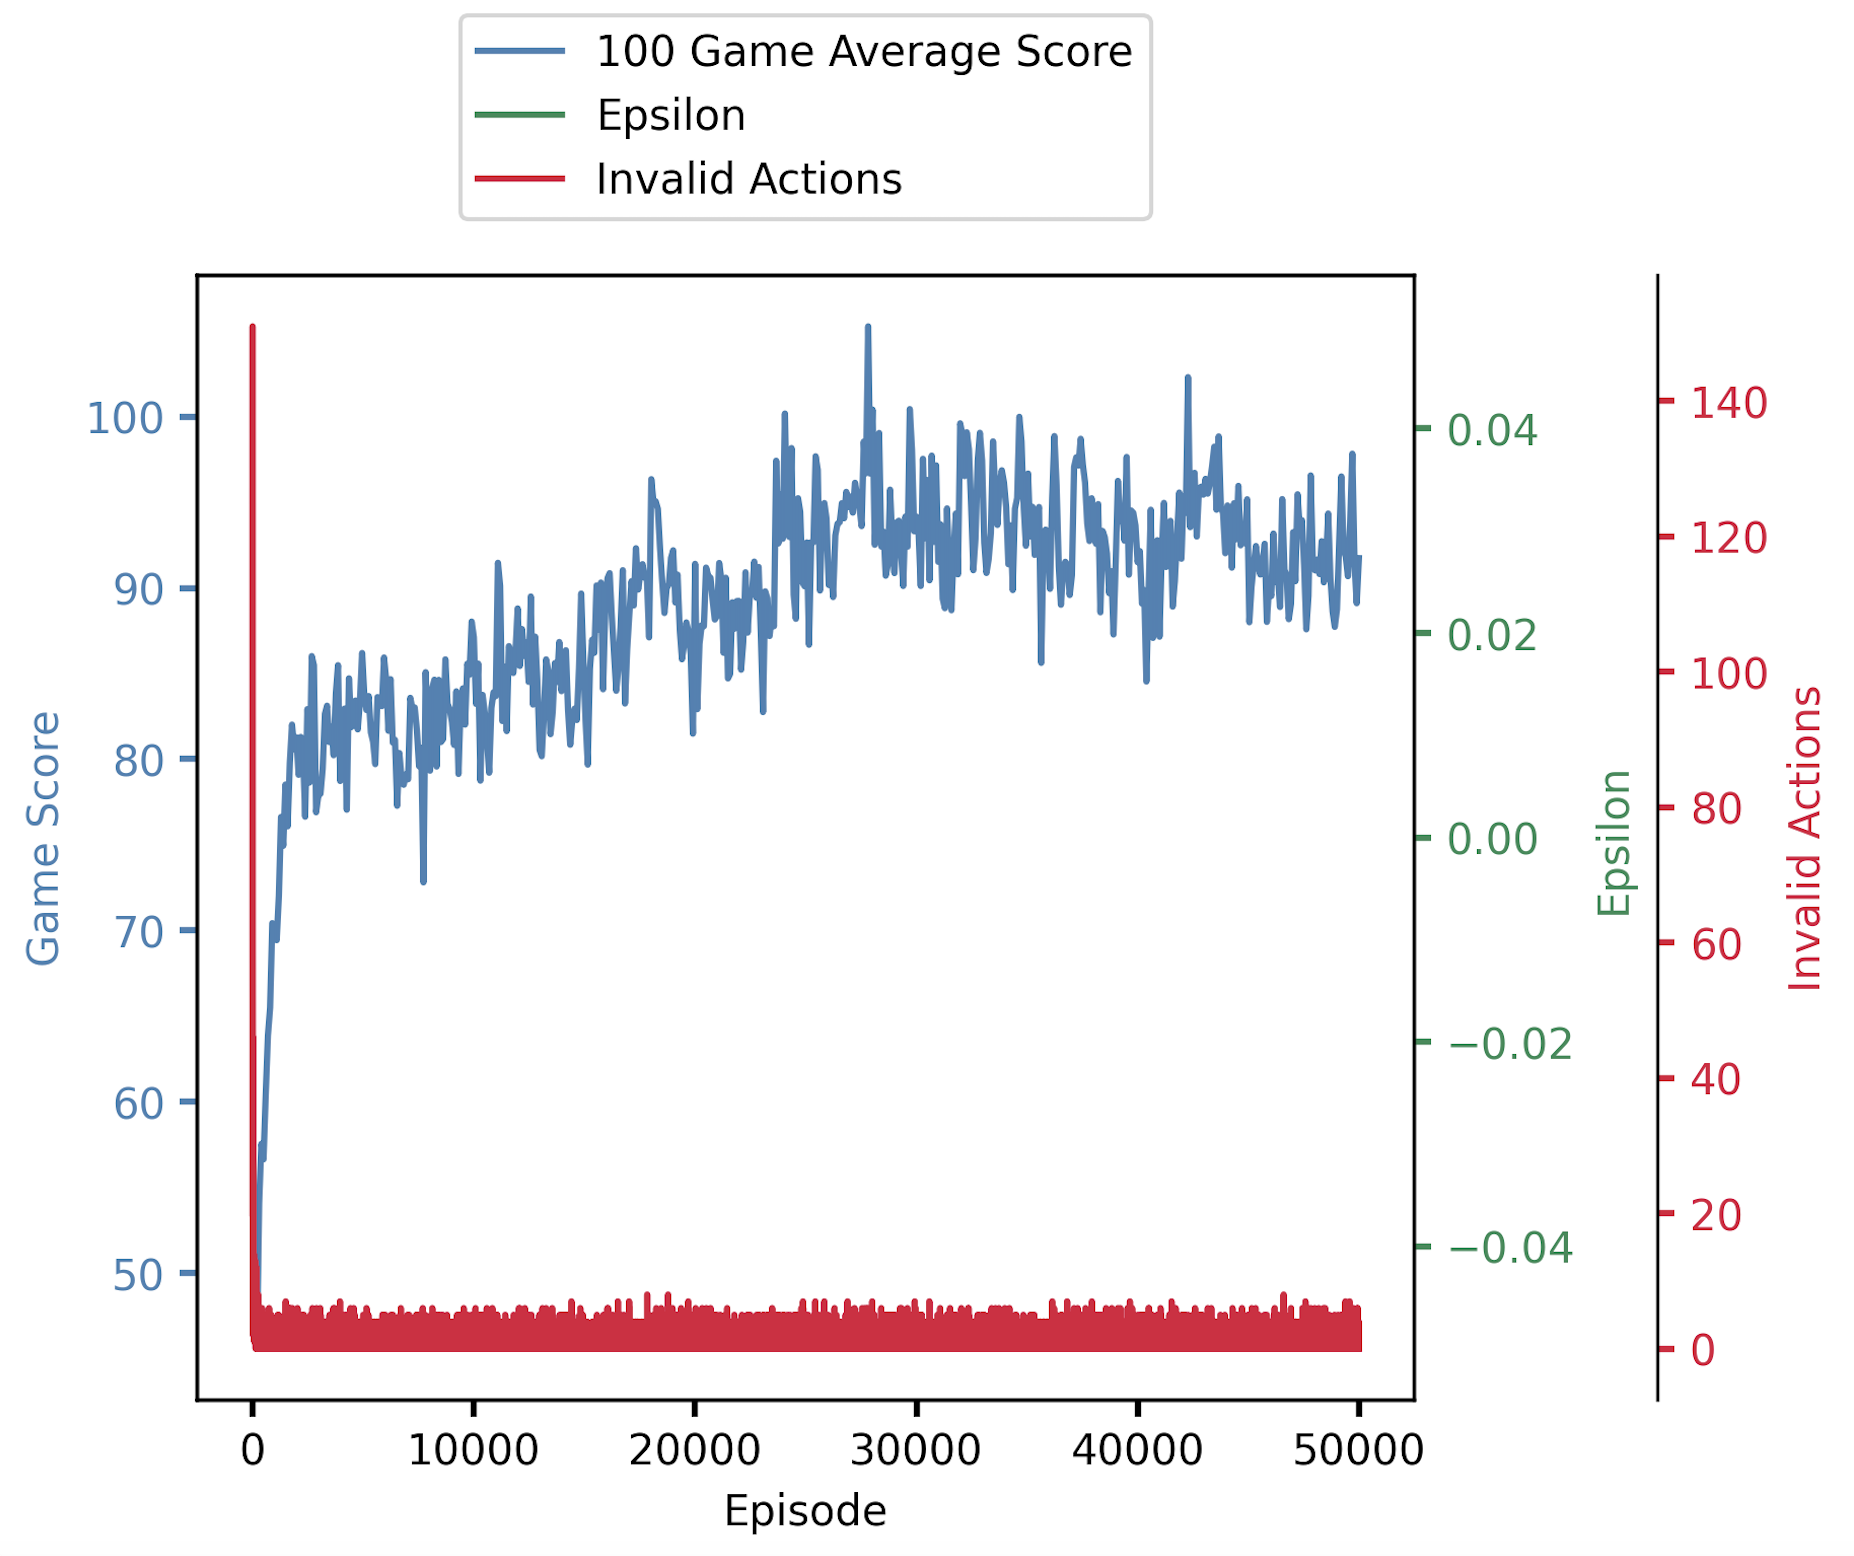
\includegraphics[width=0.3\textwidth]{naive_random} & 
        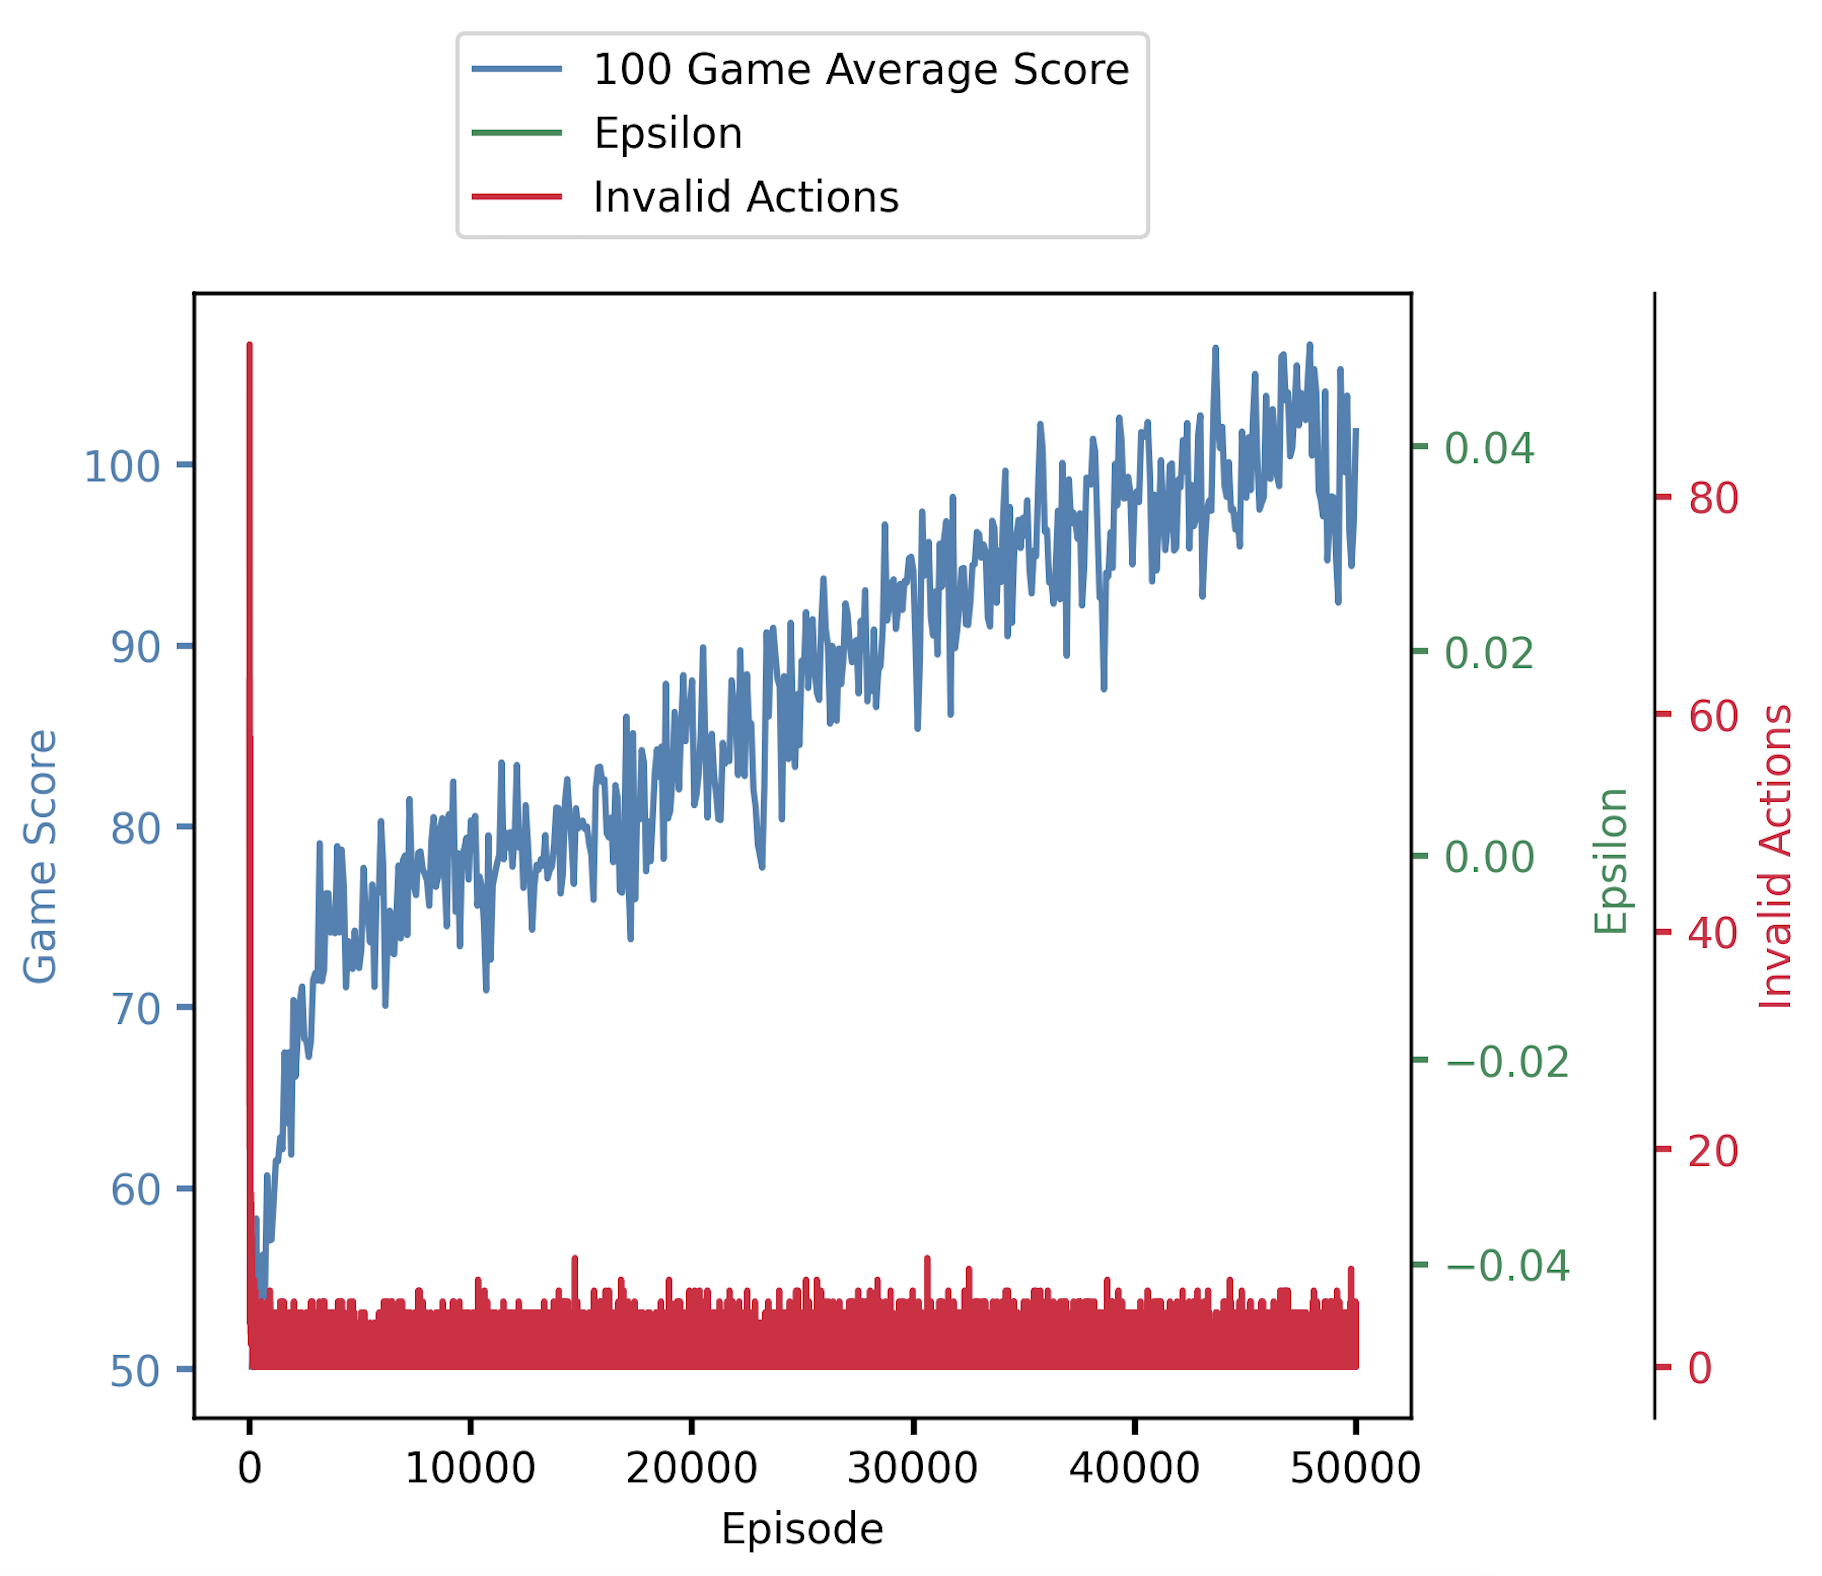
\includegraphics[width=0.3\textwidth]{naive_greedy} & 
        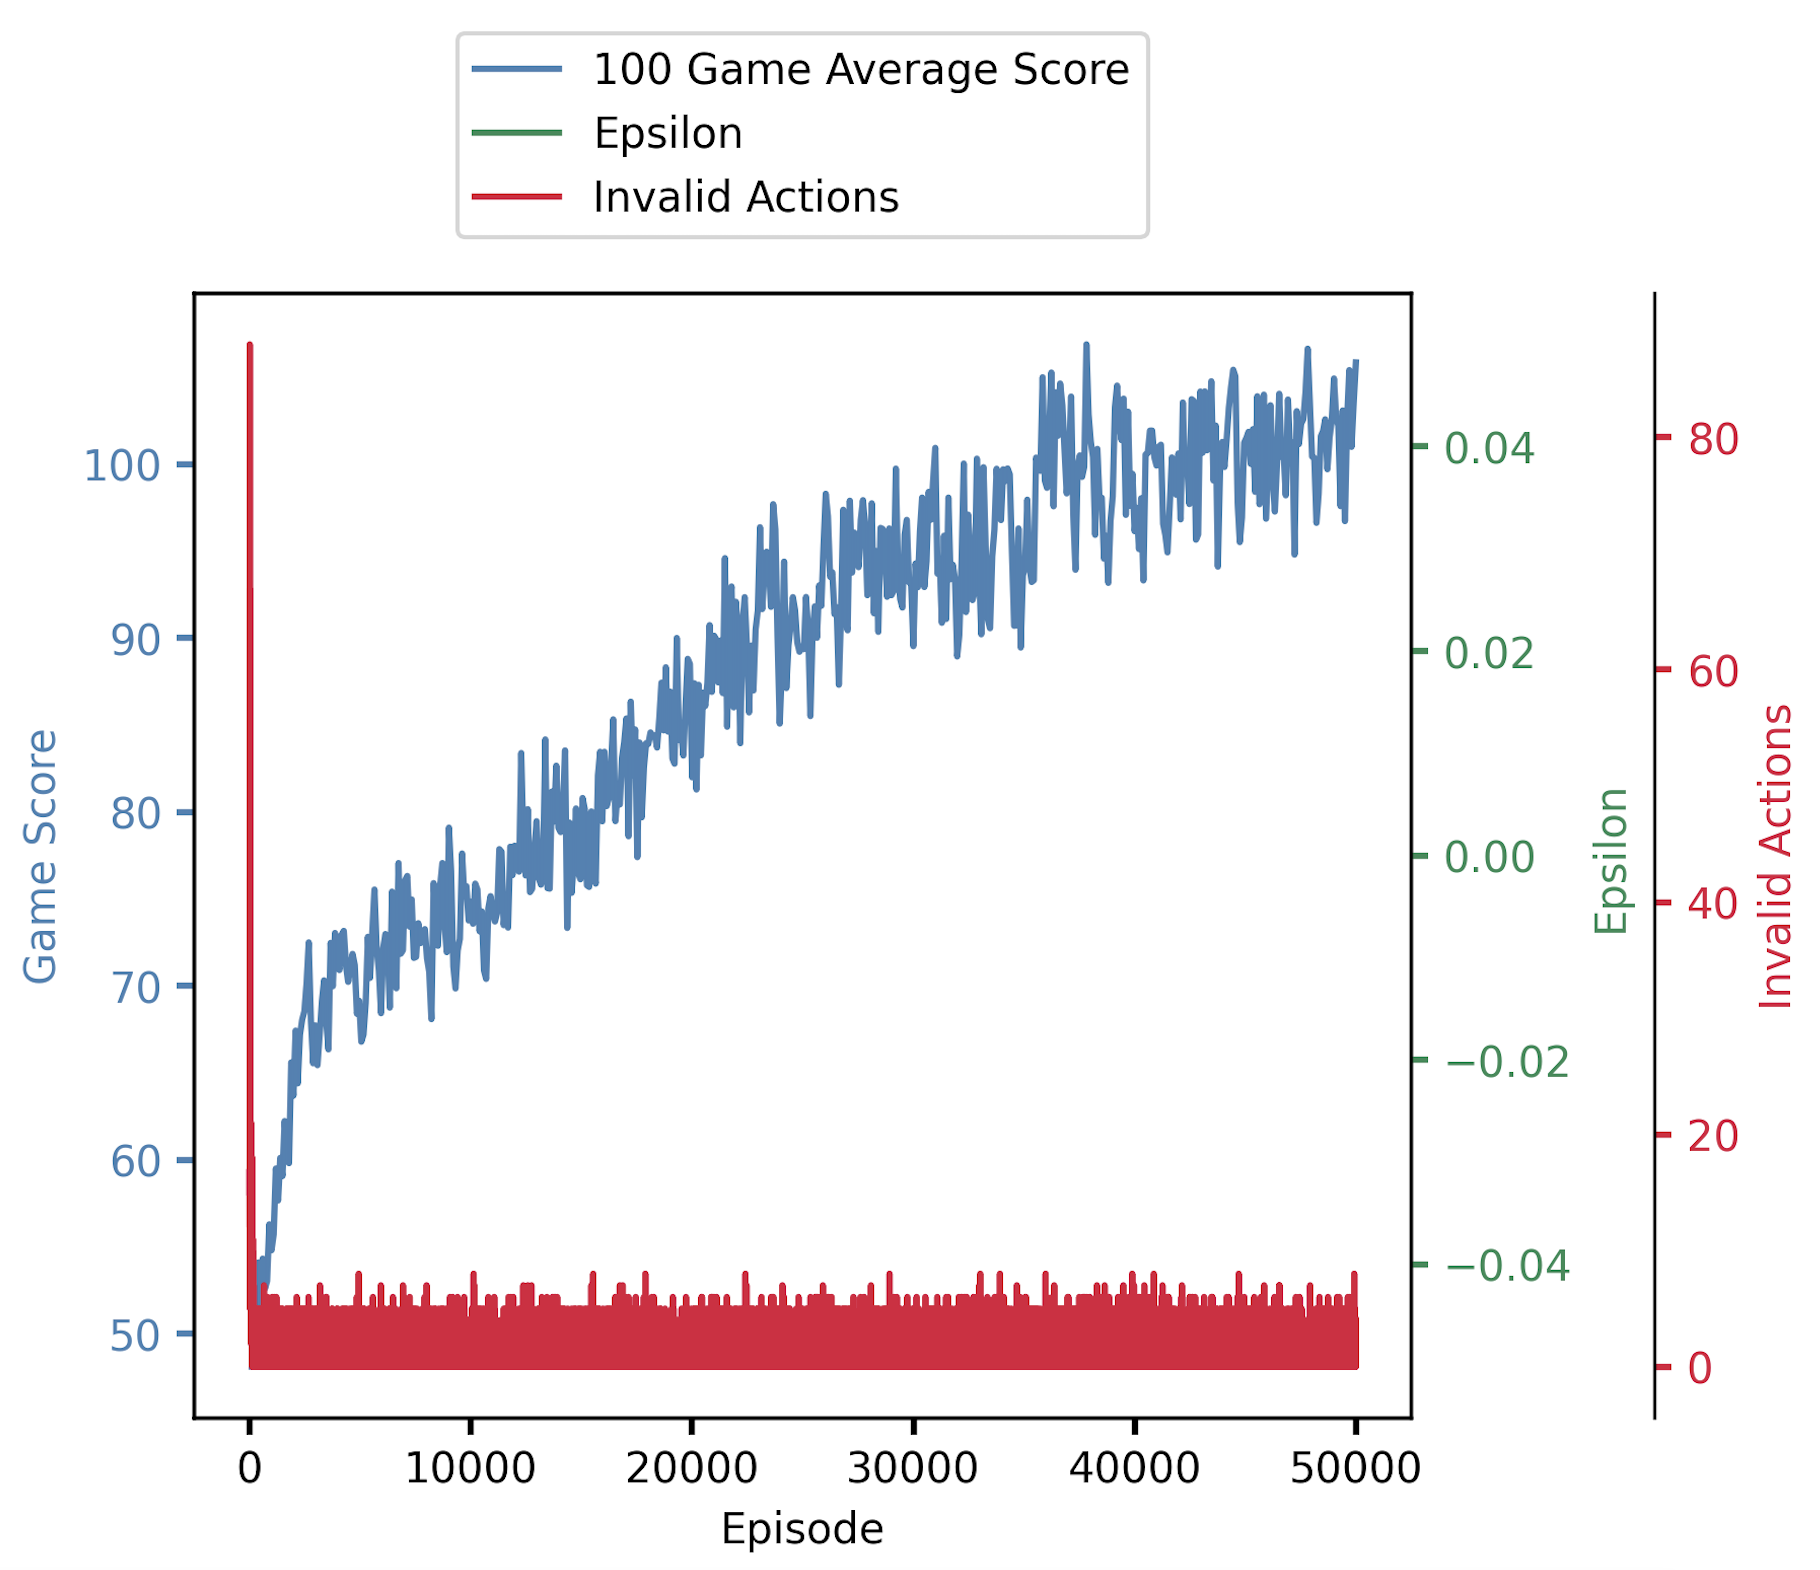
\includegraphics[width=0.3\textwidth]{naive_optimal} \\
        (a) Naive vs. Random &
        (b) Naive vs. Greedy &
        (c) Naive vs. Optimal
    \end{tabular}
\end{figure}

\begin{figure}[H]
    \begin{tabular}{cc}
        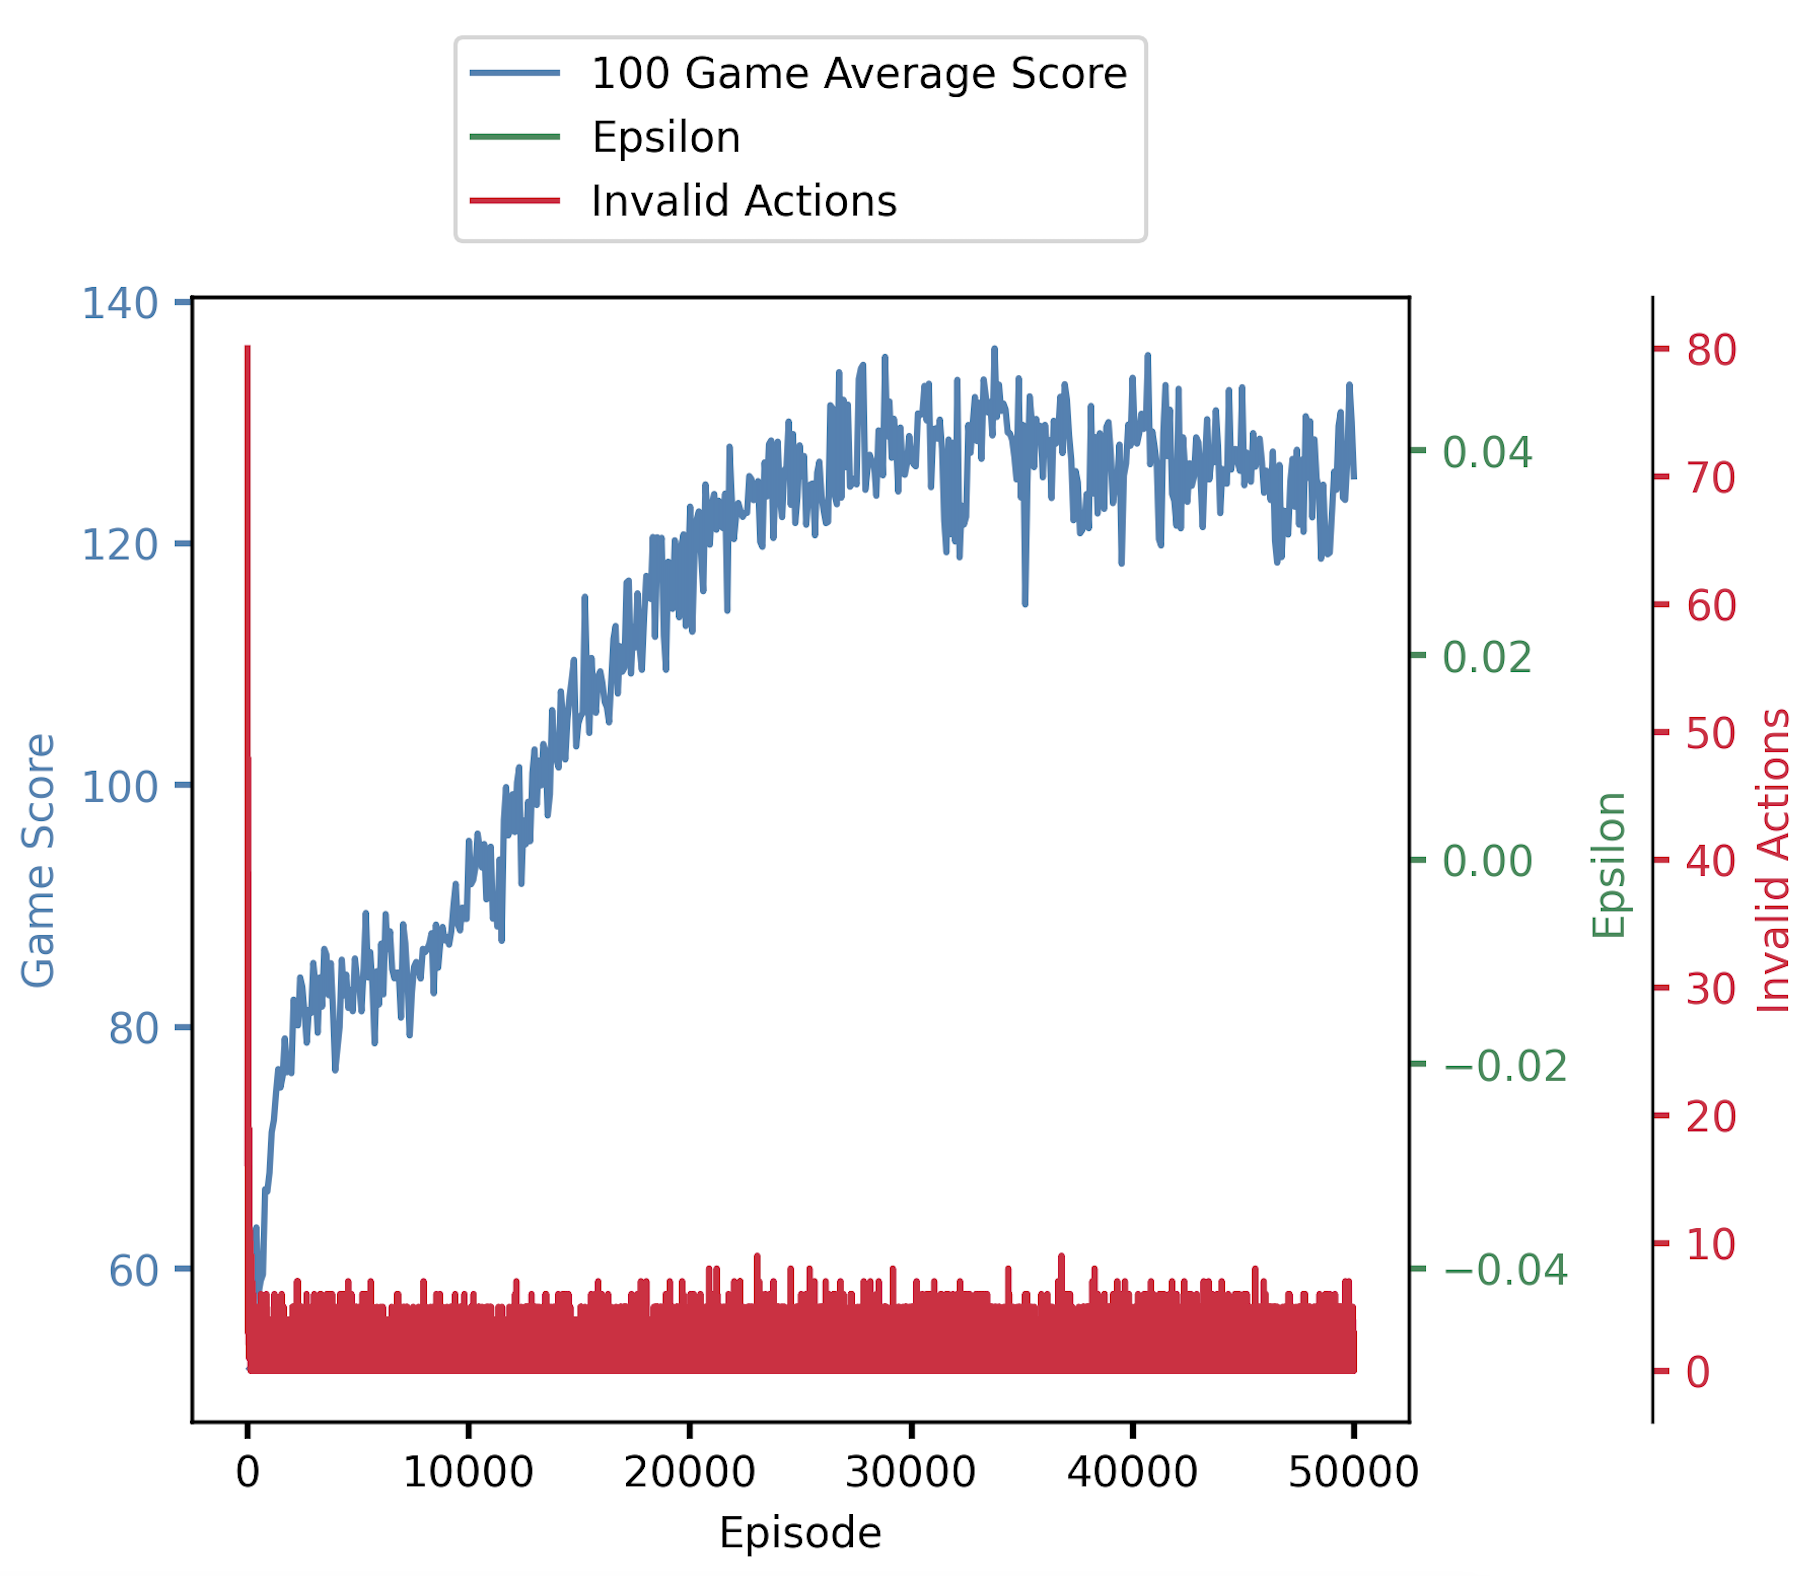
\includegraphics[width=0.45\textwidth]{gradient_greedy.png} &
        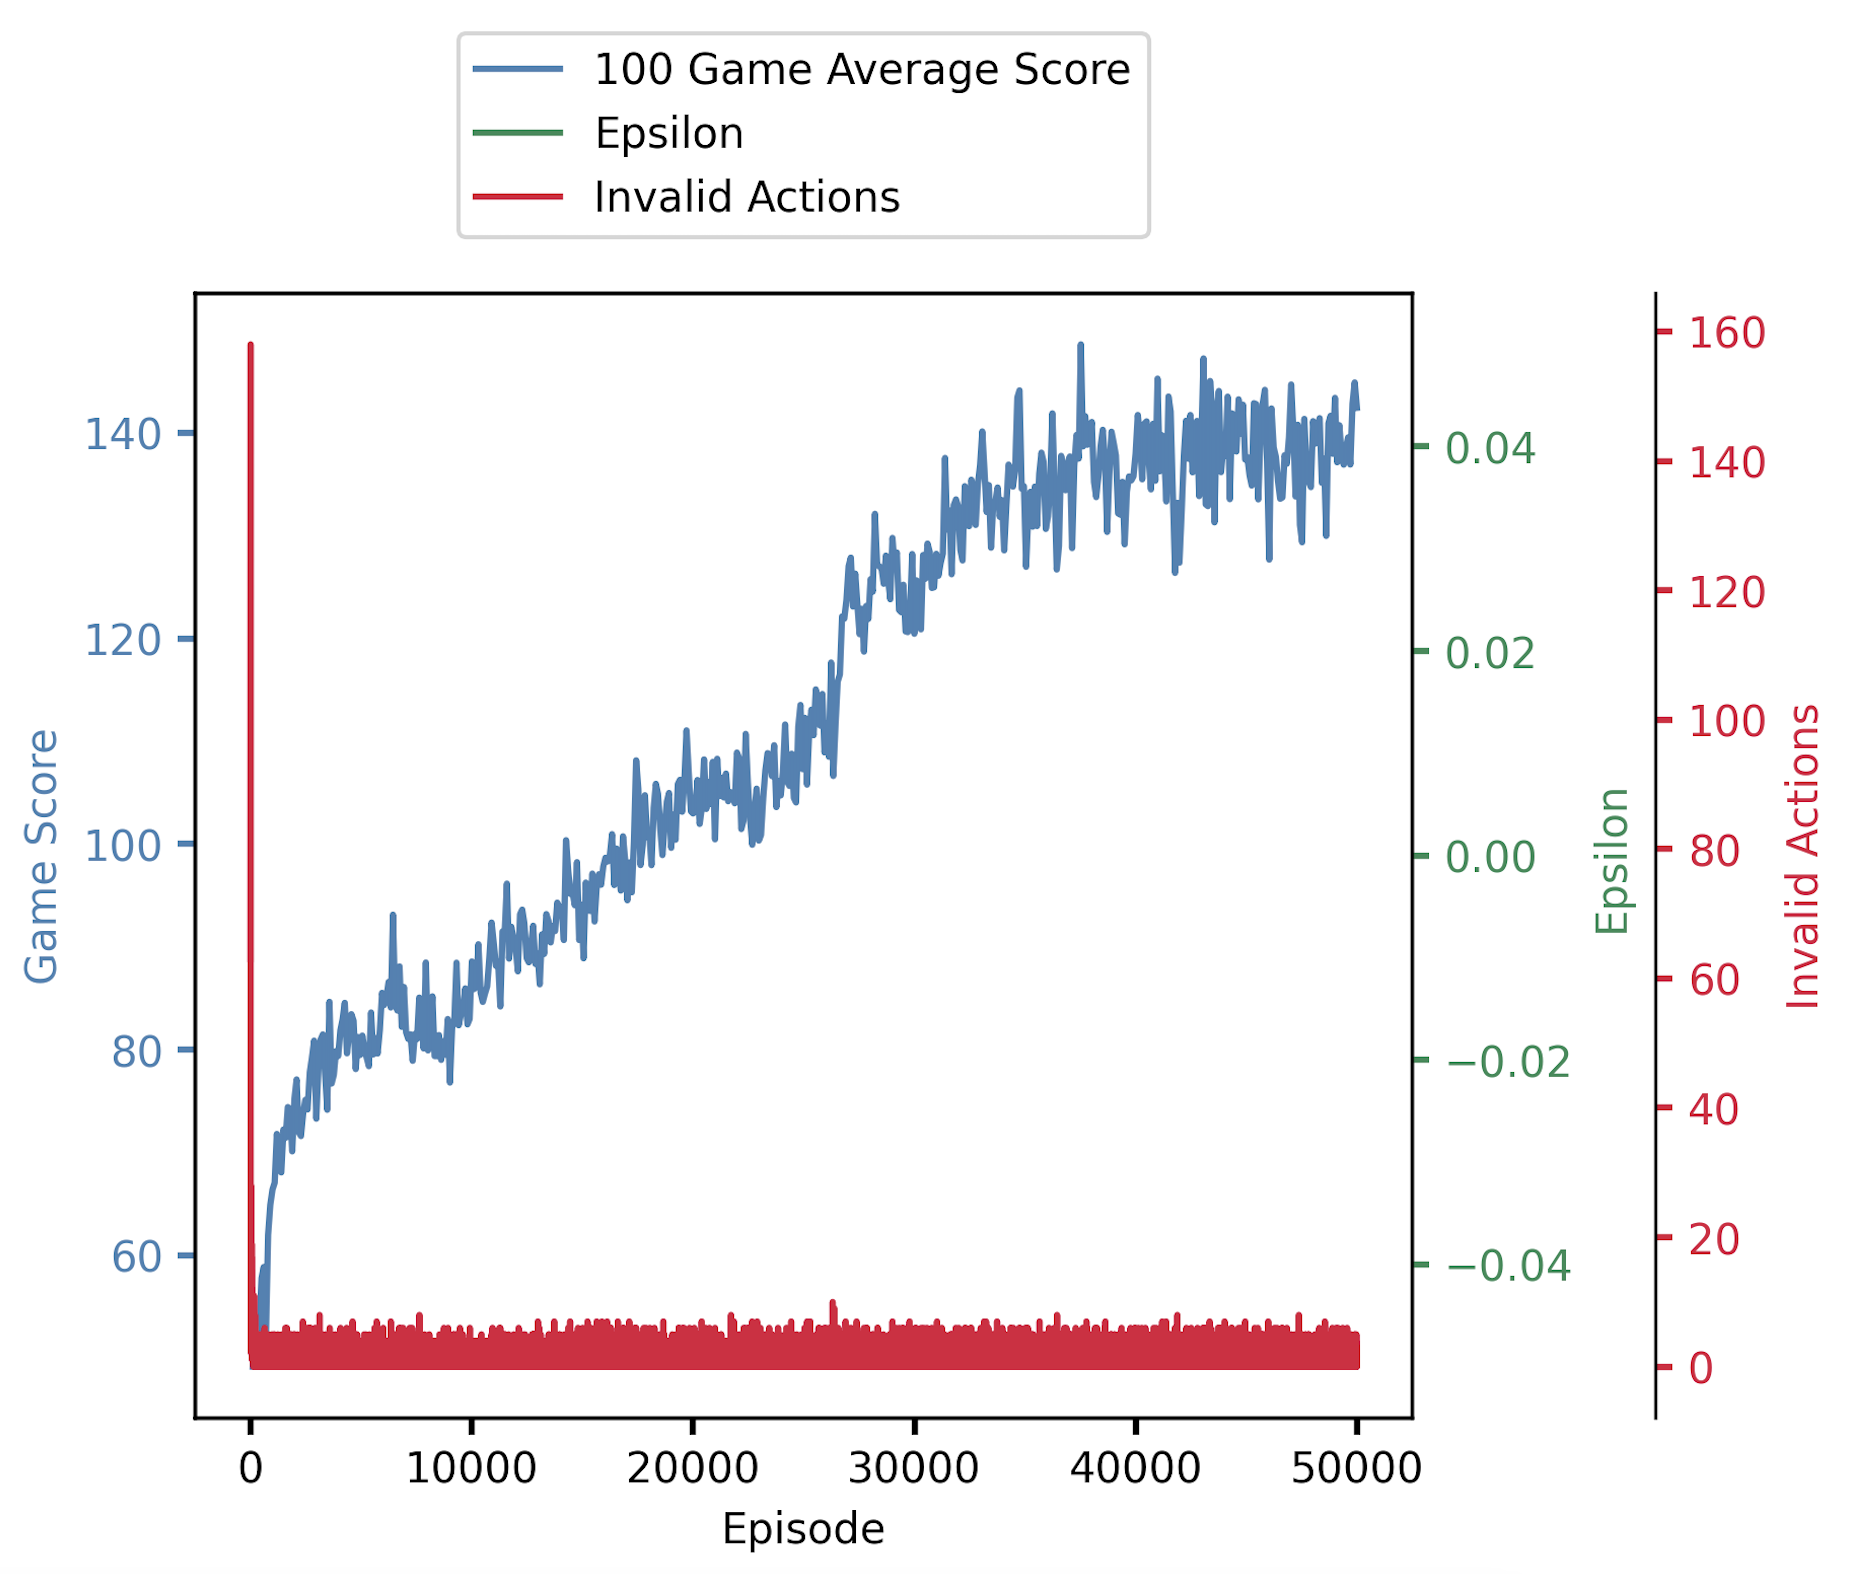
\includegraphics[width=0.45\textwidth]{gradient_optimal.png} \\
        (d) Gradient vs. Greedy 50k games &
        (e) Gradient vs. Optimal 50k games \\
    \end{tabular}
\end{figure}

\begin{figure}[H]
    \begin{tabular}{cc}
        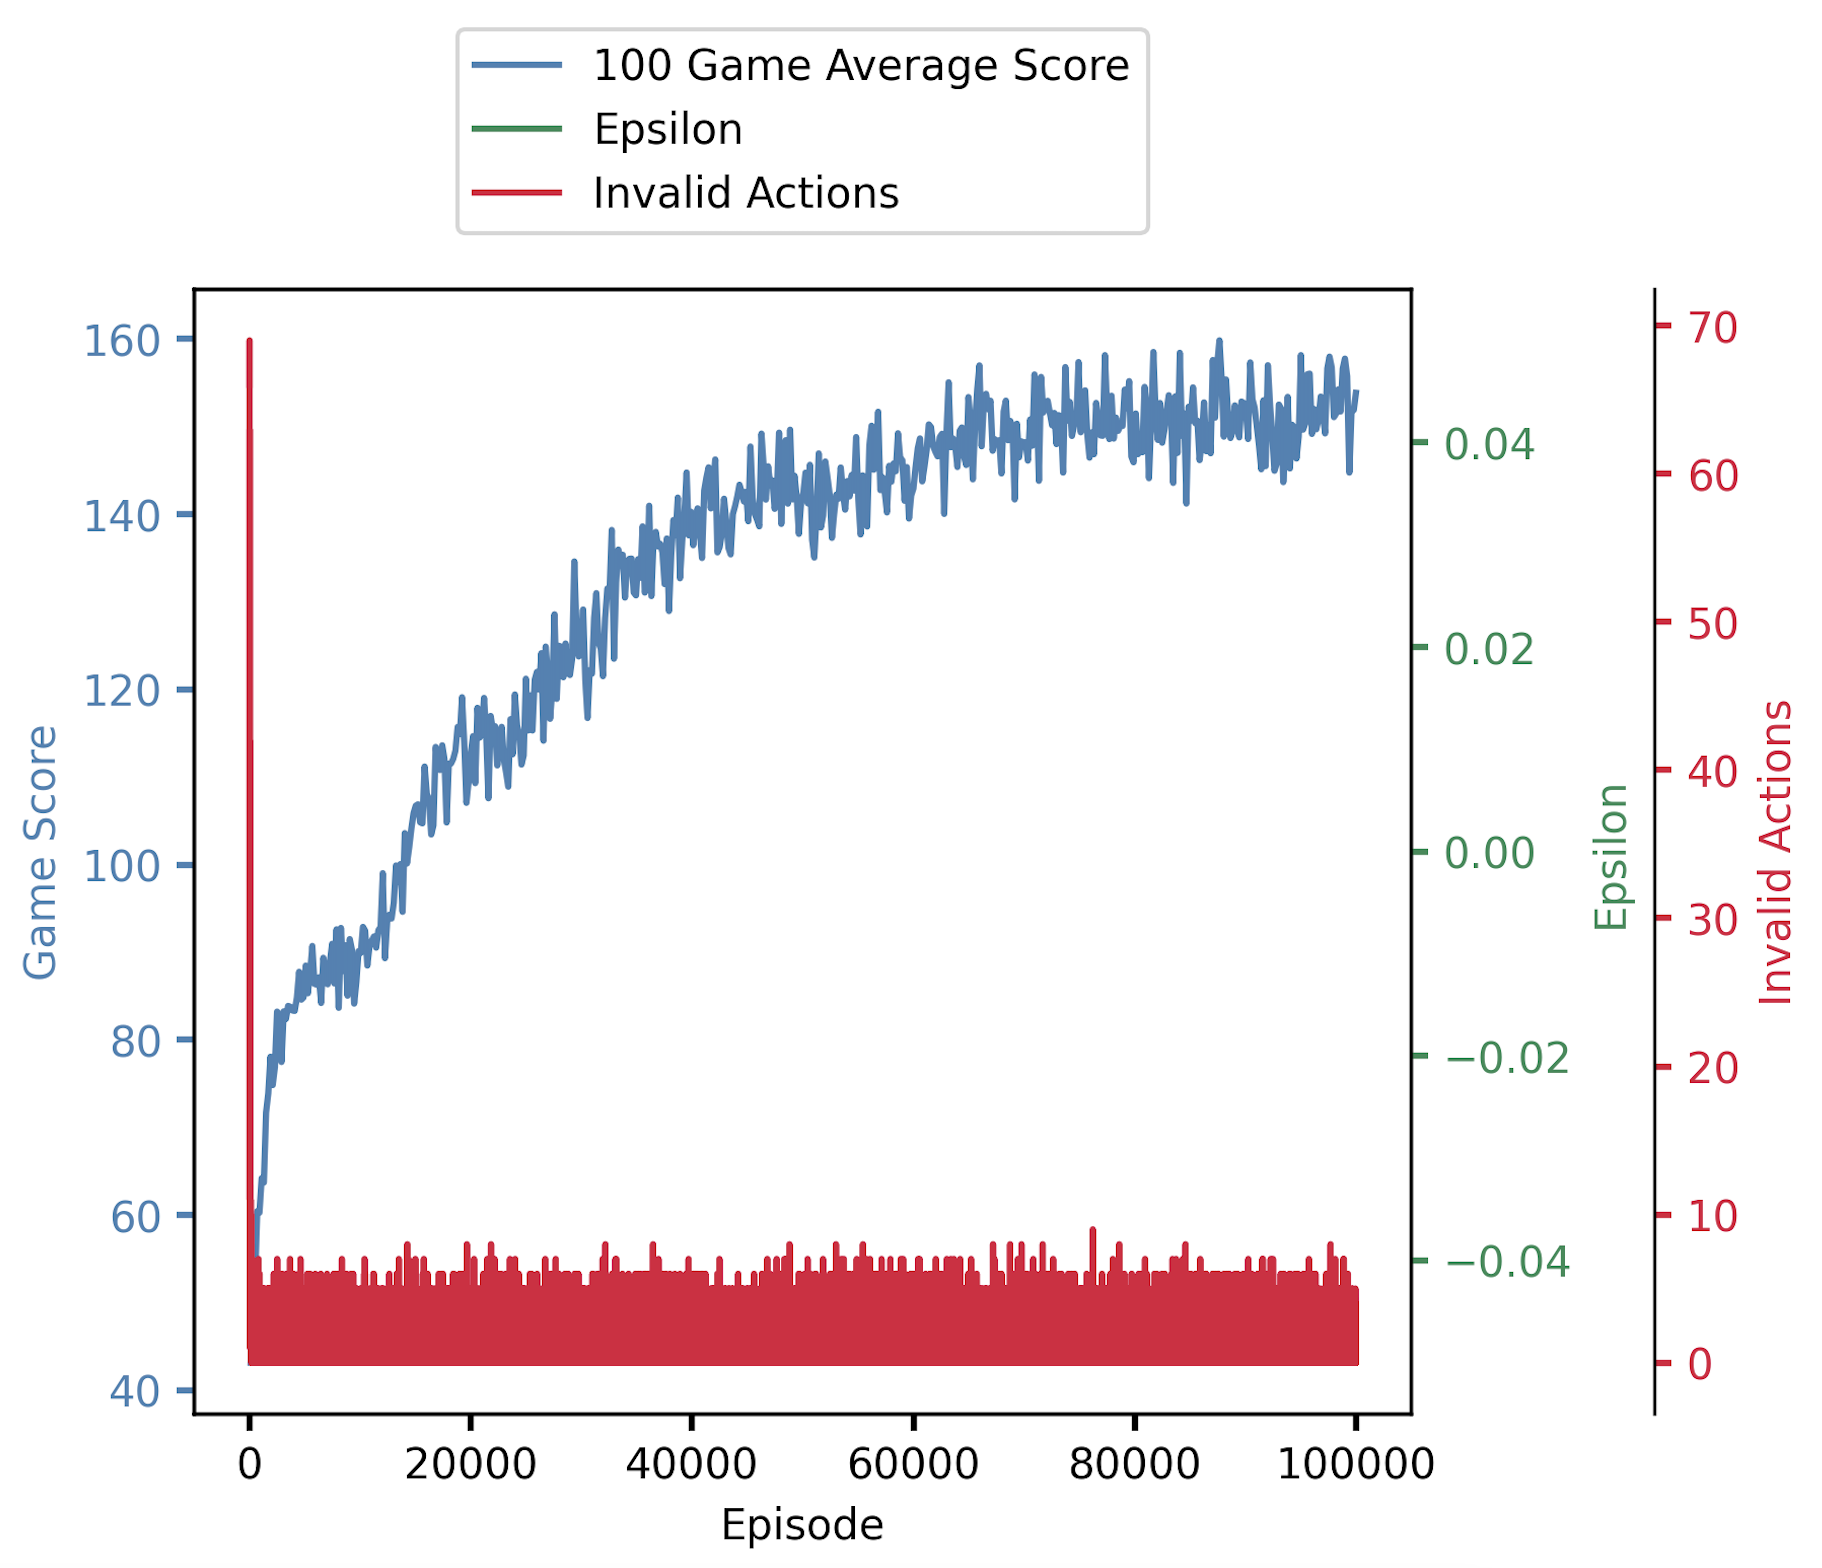
\includegraphics[width=0.45\textwidth]{gradient_greedy_long.png} &
        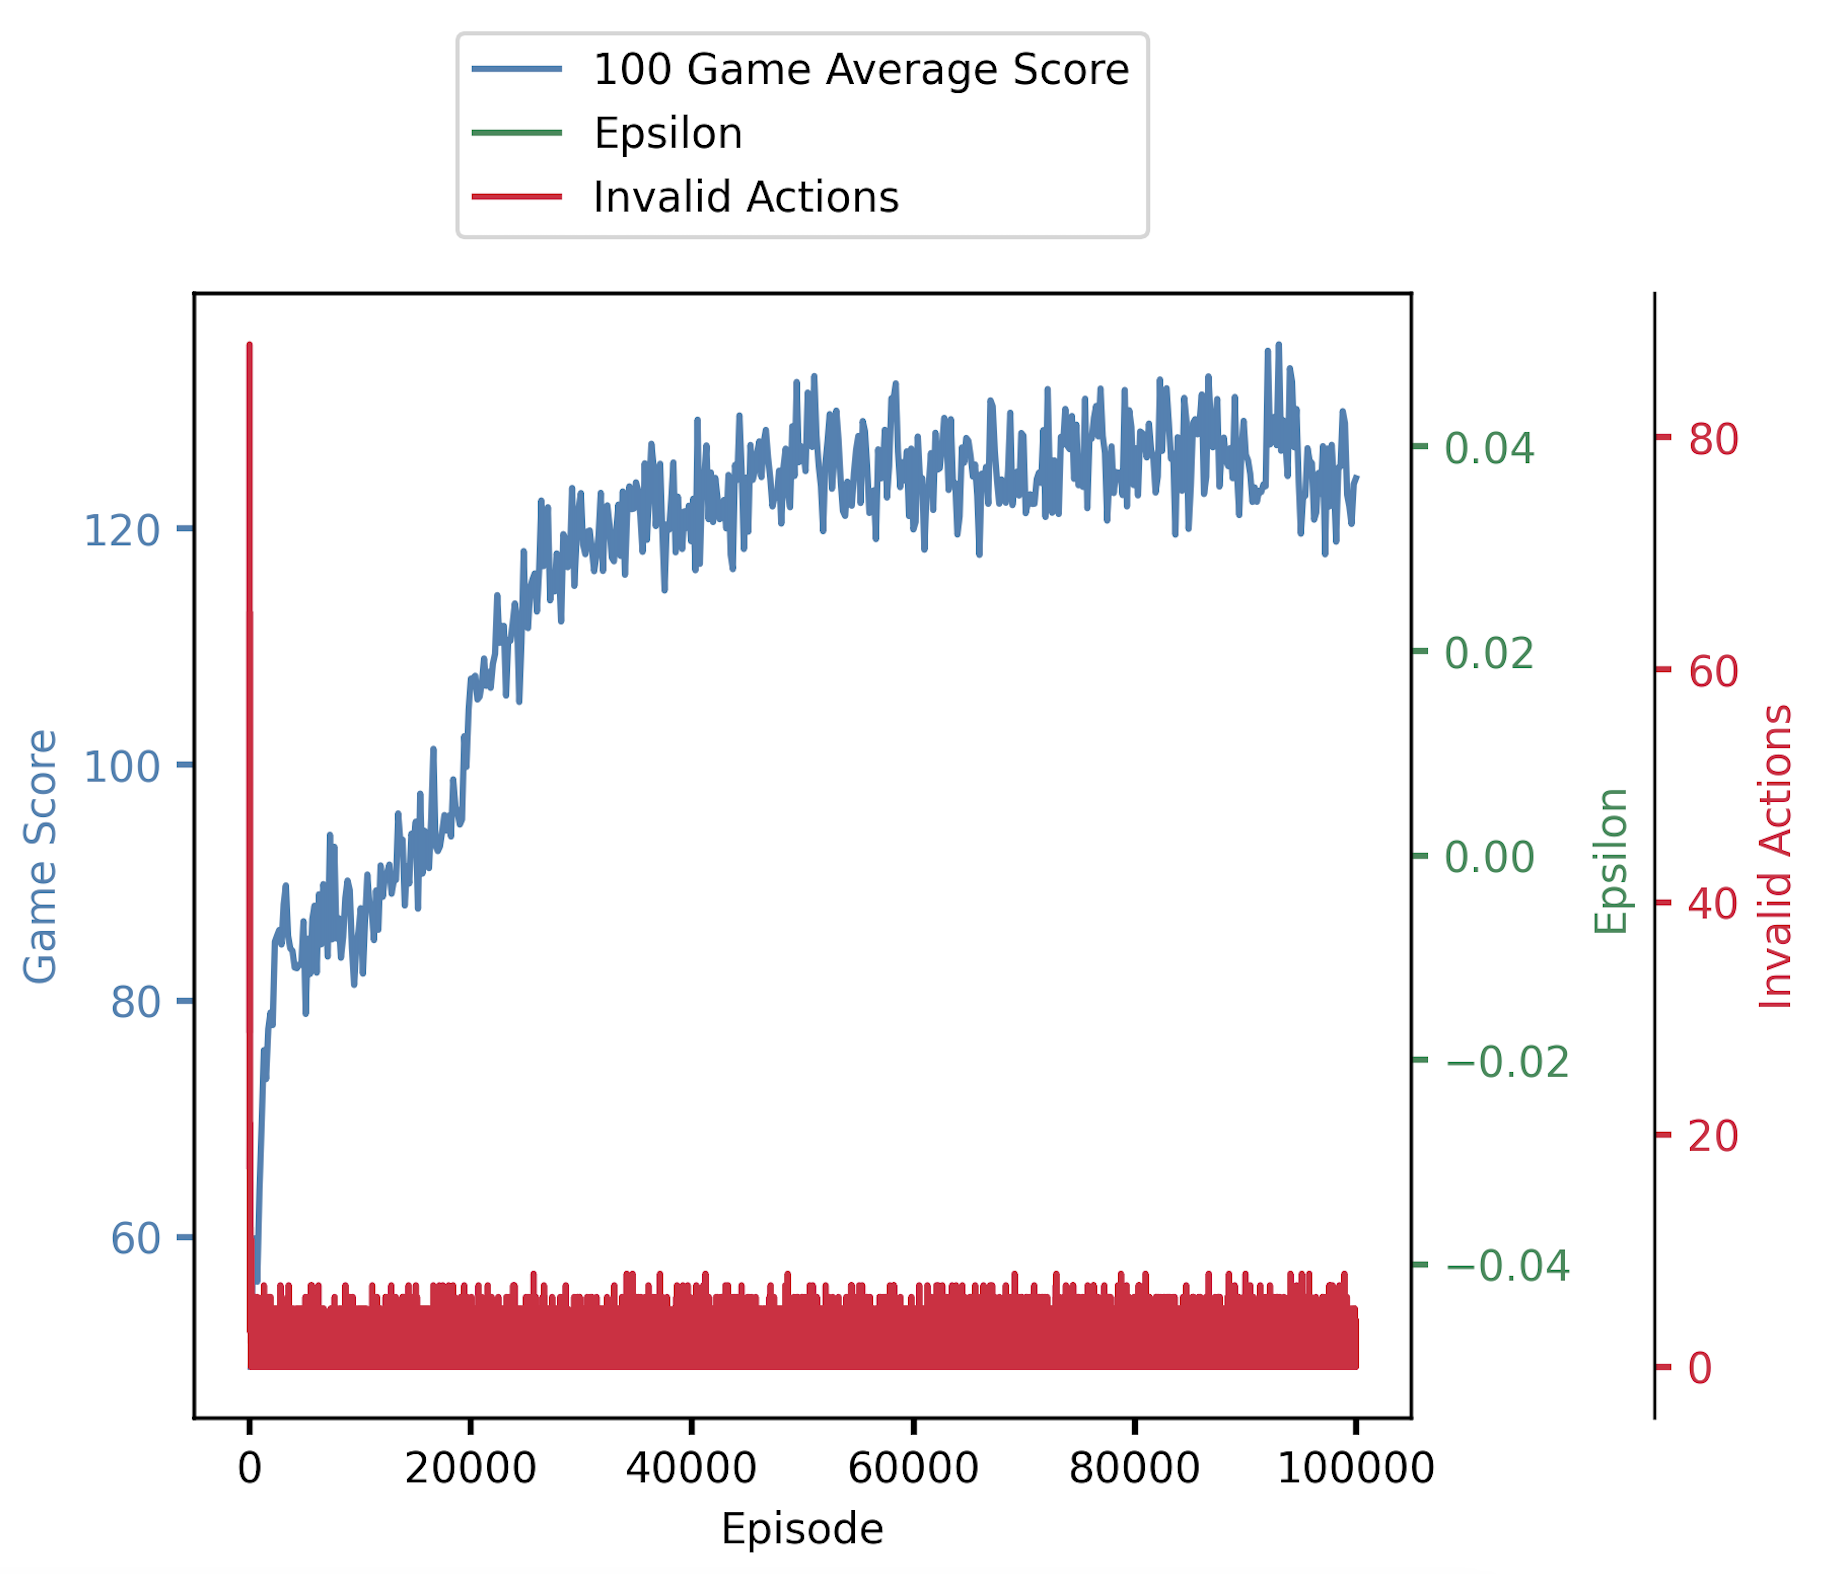
\includegraphics[width=0.45\textwidth]{gradient_optimal_long.png} \\
        (f) Gradient vs. Greedy 100k games &
        (g) Gradient vs. Optimal 100k games
    \end{tabular}
\end{figure}

\begin{figure}[H]
    \begin{tabular}{cc}
        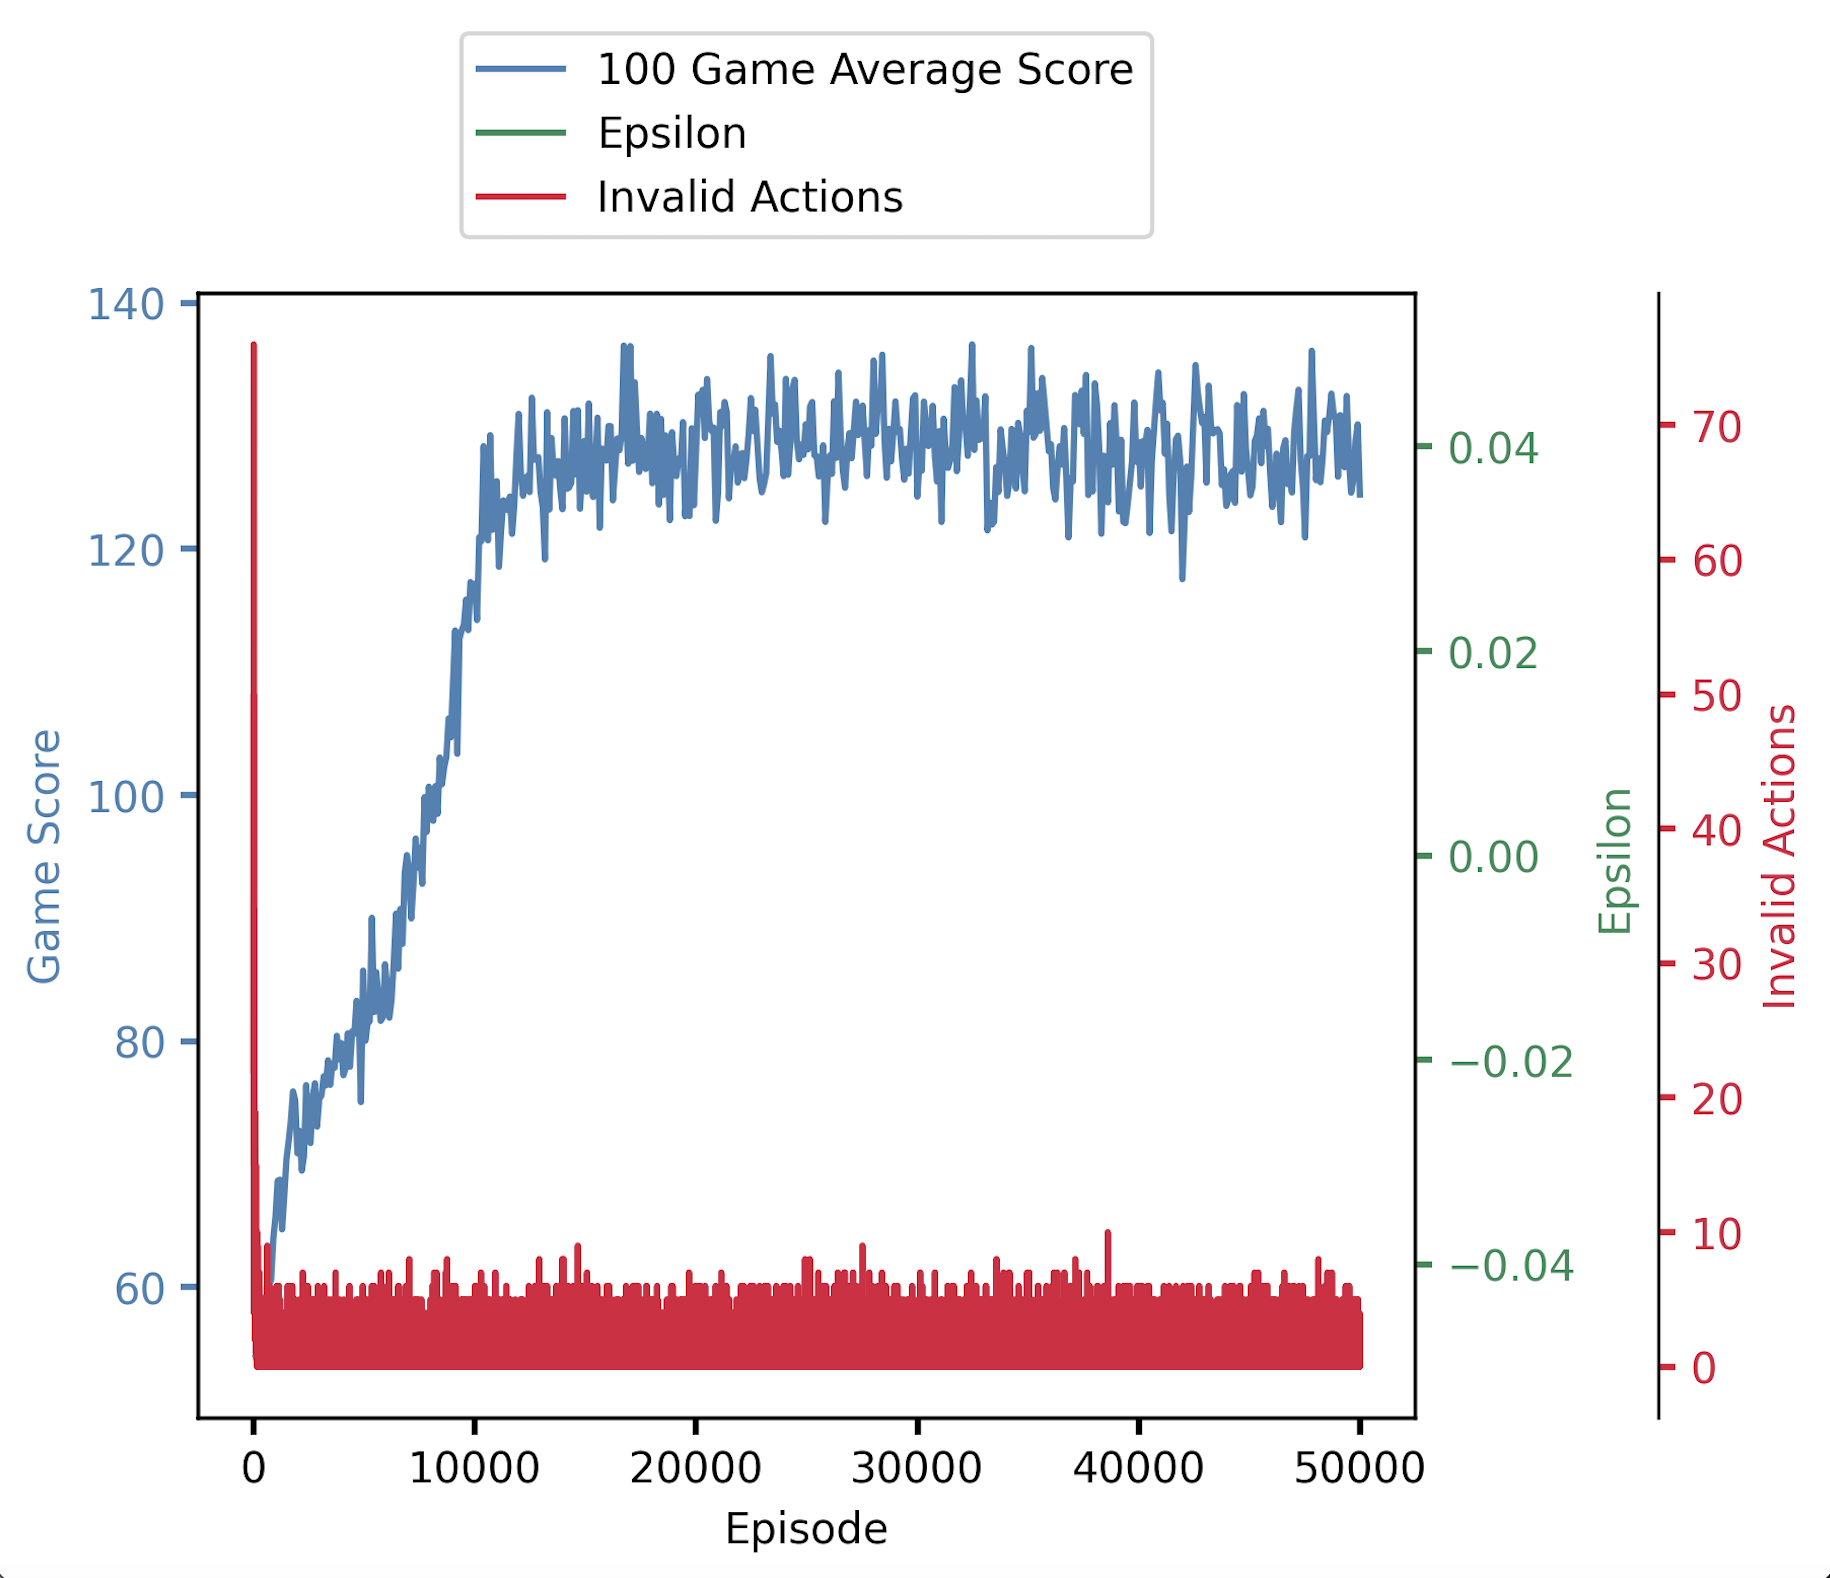
\includegraphics[width=0.45\textwidth]{fixed_random.png} &
        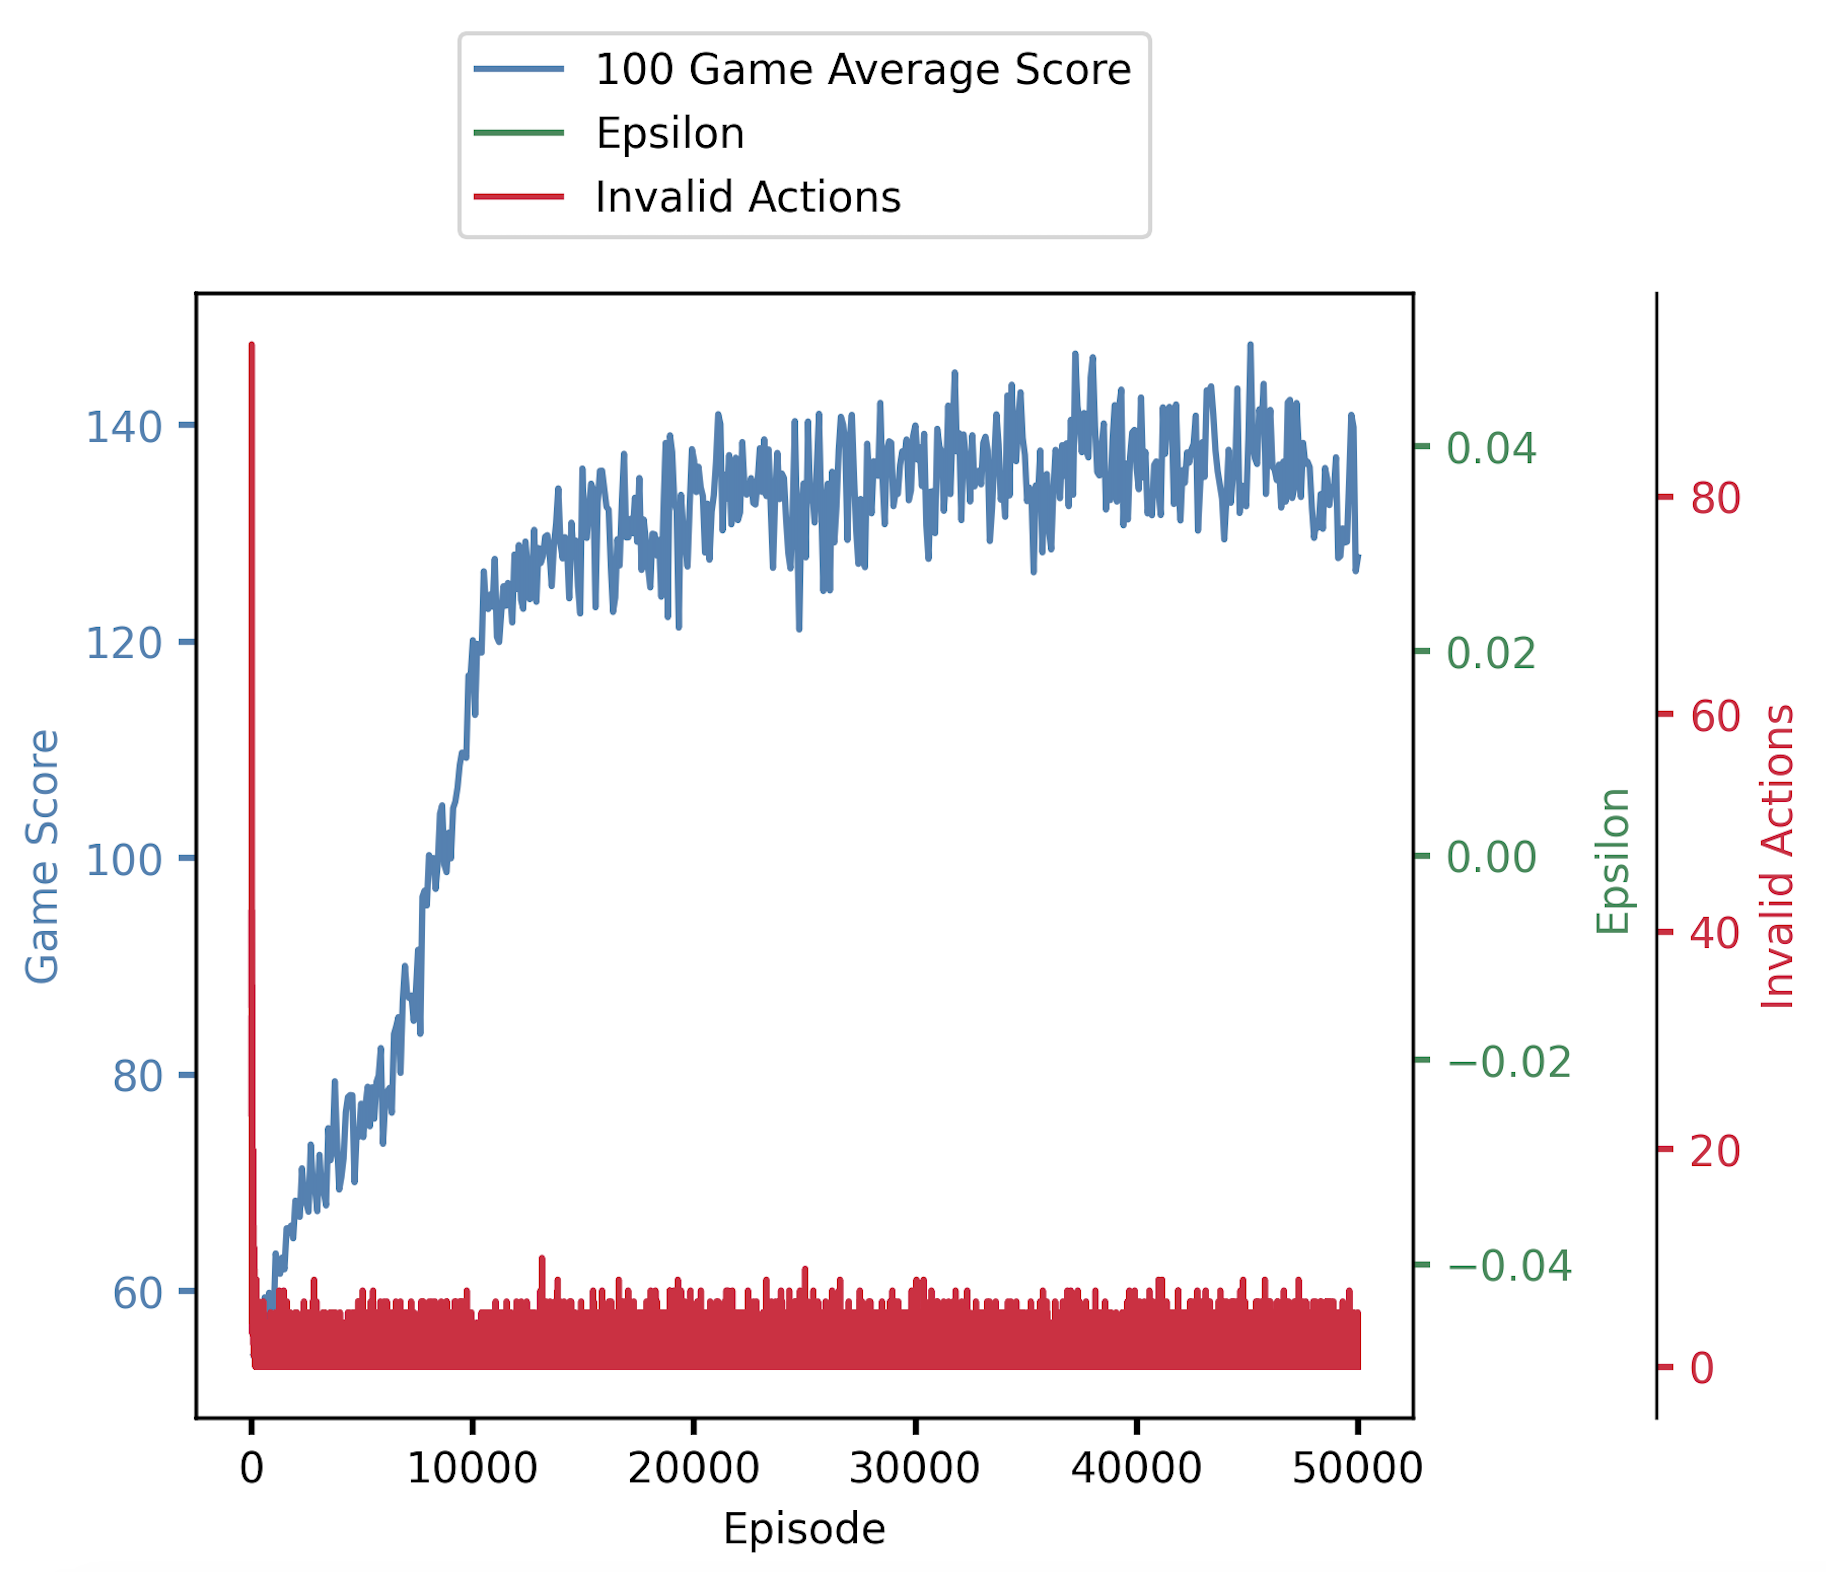
\includegraphics[width=0.45\textwidth]{flex_random.png} \\
        (h) Fixed vs. Random &
        (i) Moving Average vs. Random
    \end{tabular}
\end{figure}

\noindent
After training, each of the nine DQN agents was tested against the random, greedy, and optimal solitaire agents over the course of 10,000 games. The results are as follows:

\begin{table}[H]
    \centering
    \caption*{Average Score Over 10,000 Games}
    \begin{tabular}{ |c|c|c|c| }
        \hline
        Reward Variant - Training Opponent & Random & Greedy & Optimal \\
        \hline
        Naive - Random & 97.57 & 80.93 & 81.42 \\
        Naive - Greedy & 101.66 & 106.64 & 105.57 \\
        Naive - Optimal & 98.40 & 103.75 & 103.94 \\
        Gradient - Greedy & 127.45 & 129.22 & 124.23 \\
        Gradient - Greedy (100k) & 153.47 & 159.72 & 159.25 \\
        Gradient - Optimal & 121.13 & 143.71 & 145.47 \\
        Gradient - Optimal (100k) & 126.28 & 133.88 & 137.30 \\
        Fixed - Random & 139.44 & 134.76 & 137.28 \\
        Moving Average - Random & 144.84 & 129.45 & 131.66 \\
        \hline
    \end{tabular}
\end{table}

\begin{table}[H]
    \centering
    \caption*{Win Percentage Over 10,000 Games}
    \begin{tabular}{ |c|c|c|c| }
        \hline
        Reward Variant - Training Opponent & Random & Greedy & Optimal \\
        \hline
        Naive - Random & 94.15\% & 0.41\% & 0.14\% \\
        Naive - Greedy & 96.66\% & 0.96\% & 0.25\% \\
        Naive - Optimal & 95.42\% & 0.79\% & 0.21\% \\
        Gradient - Greedy & 99.04\% & 4.68\% & 1.17\% \\
        Gradient - Greedy (100k) & 99.73\% & 14.4\% & 6.02\% \\
        Gradient - Optimal & 99.14\% & 6.46\% & 2.88\% \\
        Gradient - Optimal (100k) & 99.09\% & 3.89\% & 1.60\% \\
        Fixed - Random & 99.56\% & 7.34\% & 2.60\% \\
        Moving Average - Random & 99.25\% & 6.09\% & 2.37\% \\
        \hline
    \end{tabular}
\end{table}

\section{Discussion}
As predicted earlier, the DQN agents employing the naive reward function where a win returns 1, a loss returns -1, and a draw returns 0, performed the worst out of all the agents. The performance against the random agent was roughly similar across the three agents, with average scores around the 100 mark and win percentages around 95\%. However, when tested against stronger opponents, the agent trained against random performed significantly worse, with average scores around 81 points. On the other hand, the agents trained against stronger opponents maintained their performance, with average scores that were even slightly higher than they were against the random agent.

In fact, it is interesting to note that all nine DQN agents had their highest average scores when tested against the agent that they were trained against. This demonstrates that the opponent's scorecard—and by extension, their strategy and performance so far in the game—influenced the learning of the DQN agent, and it optimized its playing to perform best against the specific strategy it was trained against.

In hopes of improving the performance of the DQN agent, I then trained it with the gradient reward function, where the rewards for a loss were proportional to the score difference instead of fixed at -1. This improved the DQN agent's training performance considerably, with charts (d) and (e) showing much higher average scores being obtained during training in the same amount of time as their naive counterparts. The gradient agent trained against greedy had an average score of almost 130 in its test games against the greedy agent, and the gradient agent trained against optimal had an average score of over 145 when tested against the optimal agent. The performance of the gradient agent trained against optimal also did not seem like it was plateauing at the end of the 50,000 games, so I doubled the training time to 100,000 games to see if any further improvements could be made. Surprisingly, the agent trained against greedy turned out to be the stronger player after the 100,000 games, while the agent trained against optimal performed worse when trained longer. This result highlights the nondeterministic aspect of reinforcement learning. Multiple runs with the same network and the same hyperparameters can, and likely will, lead to different results depending on the local max that the model settles on.

I then tested the two reward functions that did not rely on the opponent's score to see if they fared any better. Both the fixed and moving average variants were trained against the random agent to speed up training times. I expected the moving average variant to perform better because the score goal for the agent to beat increases as the agent learns and improves. I hypothesized that the fixed variant would plateau once it could reliably beat the set score goal of 110, while the moving average variant would continue improving. Looking at chart (h), we see that the fixed variant did indeed plateau once it could reliably beat a score of 110. However, chart (i) is not so different, showing that the moving average variant did not continue improving as expected. When tested against random, the moving average variant performed slightly better, with an average score of 144.84 compared to 139.44 for the fixed variant. However, like with the naive DQN agent, being trained against the random agent caused a significant decrease in performance when the DQN agents were tested against stronger opponents. Against greedy and optimal, it was actually the fixed variant that performed slightly better. Despite not performing as well as the gradient variant, the speed at which the fixed and moving average variants reached an average score of 120 is unparalleled. It only took around 12,000 games of training for the fixed and moving average variants to reach 120 before they started to plateau, while it took the gradient variants over double the time to do the same.

Apart from the agents' average scores during training, the charts also plot how many invalid actions were made by the agent—an indirect measure of how well the agent has learned to not choose a used category. While it is hard to tell on the graph because of how many data points there are, the number of actions quickly drops to around 0-5 invalid actions per game after roughly 200 games. For the majority of games, in fact, the number of invalid actions is just zero or one after the first 200 games.

Overall, the best-performing DQN agent was the one that trained for 100,000 games against the greedy agent using a gradient reward function. It had the highest average scores when tested against all three types of opponents, and it also held the highest win percentages against all opponents. Still, its performance was disappointing, with only a 14.4\% winrate over a player playing a greedy solitaire strategy and only a 6.02\% winrate over a player playing the optimal solitaire strategy. While the goal of this project was to develop a DQN agent that could compete with the optimal solitaire strategy in a 2-player setting, more work is required to fine-tune the neural network's architecture and hyperparameters along with my custom Yahtzee environment's observation space and reward function.

\section{Future Work}
My implementations of the deep Q-Learning network and its corresponding Yahtzee gym environment are easily customizable to test different network architectures, hyperparameters, and reward functions. Spinning up a new opponent agent to test the model against is also incredibly straightforward with my implementation. With more time, the DQN agents could be trained for even longer, perhaps one million games, in order to realize their full potential. In order to optimize performance, the various hyperparameters would all have to be tuned, and the architecture itself might have to be modified. The number of hidden layers, size of each hidden layer, activation functions, and even a type of neural network that is not just a simple feed-forward network should all be tested to see what combination works best. Most importantly, however, I would spend more time developing various reward functions and playing with the environment's observation space to figure out how to best nudge the agent in the right direction during training and determine if it needs more or less information about the game state. Perhaps a combination of the gradient and moving average variants is better than the two on their own, where the model first trains using the moving average variant for its fast initial learning speed and then switches to the gradient variant for sustained improvement. Or, perhaps the DQN would be better off if it was given more information about the dice, such as the sum of the dice. 



\newpage

\section{References}
\printbibliography[heading=none]

\end{document}
